\documentclass[a4paper,10pt]{article}

\usepackage[T1]{fontenc}
\usepackage[utf8]{inputenc}

\usepackage{amsmath}
\usepackage{amssymb}

\usepackage{xcolor}
\usepackage{graphicx}
\usepackage{grffile}

\usepackage{subcaption}

\usepackage{booktabs}

\title{Bayesian Sparsification of $\cplx$-valued networks}
\author{Ivan Nazarov, and Evgeny Burnaev}

%% notation
\newcommand{\real}{\mathbb{R}}
\newcommand{\cplx}{\mathbb{C}}
\newcommand{\tr}[1]{\mathop{tr}{#1}}

\newcommand{\hop}{{\mkern-1.5mu\dagger}}
\newcommand{\conj}[1]{\overline{#1}}

% \renewcommand{\top}{{\mkern-1.5mu\intercal}}
\renewcommand{\vec}[1]{\overrightarrow{#1}}
\newcommand{\diag}[1]{\mathrm{diag}{#1}}

%% drafting macro
\newcommand{\important}[1]{\textbf{\!\colorbox{red}{#1}\!}}
\newcommand{\attn}[2]{\textbf{\color{red} #2~\textsuperscript{\textit{[#1]}}}}
\newcommand{\verify}[1]{\textit{\!\colorbox{red}{#1}\!}}
\newcommand{\rewrite}[1]{\attn{rewrite}{#1}}
\newcommand{\todo}[1]{{\color{blue} [TODO]} \important{#1}}

%% red-highlight missing citations
\usepackage{etoolbox}
\makeatletter
\patchcmd{\@citex}{\bfseries ?}{\colorbox{red}{\bfseries ?}}{}{}
\makeatother

\begin{document}
\maketitle

\section{Introduction} % (fold)
\label{sec:introduction}

Deep neural networks are an integral part of machine learning and data science toolset
for practical data-driven problem solving. Despite recent advances in generalization
and optimization theory specific to deep networks, deploying in actual embedded hardware
remains a challenge. Solving the storage and compute constraints encourages development
of model compression and sparsification methods, that focus on favourable tradeoff between
performance and size. Most popular techniques include weight pruning \cite{citation_needed},
model quantization from IEEE754 floating point to integer-based arithmetic \cite{citation_needed},
and dropout. The key assumption is that the more explicitly zero parameters there is,
the less computations is needed.

Bayesian Inference is a principled framework of reasoning about uncertainty. The core principle
is updating prior beliefs in accordance with the likelihood of empirical observations into
posterior belief. Under suitable modelling and prior assumptions, Bayesian methods can be
used towards model sparsification, \cite{kingma_variational_2015,molchanov_variational_2017},
and \cite{kharitonov_variational_2018}.

% complex nets and related stuff
data that is naturally complex-valued
studies have shown a potentially richer representation of complex nets
\cite{hirose2003,fijulamin2009}
% [3] Akira Hirose, Complex-valued neural networks: theories and applications, vol. 5, World Scientific, 2003.
% [4] Md Faijul Amin and Kazuyuki Murase, “Single-layered complex-valued neural network for real-valued classification problems,” Neurocomputing, vol. 72, no. 4-6, pp. 945–955, 2009.

the complex version of backpropagation algorithm  was proposed because of
its richer representational capacity.
% Nevio Benvenuto and Francesco Piazza, “On the complex backpropagation algorithm,” IEEE Transactions on Signal Processing, vol. 40, no. 4, pp. 967–969, 1992.


\cite{yang_complex_2019} develop complex transformer, with $\cplx$-attention and complex
encoder-decoder, and apply it to music transcription and wireless signal classification.

that interfaces the rest of
$\cplx$-valued
the network with complex numbers


that operates on the Fourier transform input speech, acoustic, of radio signals.


papers related to complex-valued distributions \cite{pav_moments_2015,taubock_complex-valued_2012},
and \cite{karseras_caution:_2014}

Application of complex-valued networks is not new, \cite{citation_needed}. More recently
they were applied to music transcription and speech recognition \cite{trabelsi_deep_2017},
and \cite{yang_complex_2019}. The key motivation behind adoption of $\cplx$-networks is
pervasiveness of $\cplx$-valued data in digital signal processing \cite{citation_needed},
acoustic and radio signal analysis \cite{citation_needed}, and quantum systems modelling
\cite{citation_needed}, etc. All these applications require compliance with algebraic
operations in the field of complex numbers.


The paper is structured as follows. In sec.~\ref{sec:bayesian_dropout} we review Bayesian
dropout techniques, and ins sec.~\ref{sec:c_valued_networks} we provide a brief summary of
the inner working of complex-valued networks as functions of complex argument. The main
contribution of this study is presented in sec.~\ref{sec:dropout_for_c_valued_layers},
where we consider different variational approximations and priors, outline the tricks
and derive expressions for the divergence term. In sec.~\ref{sec:experiments} we evaluate
the sparsification rate and compare the resulting performance of various $\cplx$-networks
proposed in prior work, and discuss the outcomes in sec.~\ref{sec:discussion_and_related_research}.

% section introduction (end)


\section{Bayesian Dropout} % (fold)
\label{sec:bayesian_dropout}

In general, the core of Bayesian Inference can be summarized as follows: given a prior
distribution $\pi(m)$ on models (hypotheses) $\mathcal{M}$, utilize the empirical evidence
$D$ to update the assumptions by considering the likelihood of the observations under each
$m \in \mathcal{M}$. Models are represented by a parametric family indexed by $\omega \in
\Omega$ and each $m_\omega(\cdot)$ specifies the conditional distribution of the data $
  D = (z_i)_{i=1}^N
$. The posterior distribution $p(\omega \mid D)$, derived using the Bayes rule $
  p(m \mid D) = \tfrac{p(D \mid m) \pi(m)}{p(D)}
$ with $
  p(D) = \mathbb{E}_{\pi(m)} p(D \mid m)
$, provides useful information about yet unobserved data and model parameters, e.g
classification uncertainty, predictive statistics, and parameter relevance.

The posterior itself is computationally intractable, save for the relatively simple cases
\cite{citation_needed}, and therefore exact inference is traded for tractability and scalability
of Variational Inference. Instead of deriving $p(\omega \mid D)$ using the rule, this approach
recasts posterior inference into variational optimization problem: finding $q$ that is close
to $p(\omega \mid D)$ in terms of a proximity score $\rho$
\begin{equation}  \label{eq:variational-progam}
  q_*
    \in \arg \min_{\theta} \rho\bigl(
      q_\theta(\omega), p(\omega \mid D)
    \bigr)
    \,,
\end{equation}
over a tractable parametric family of distributions on the parameter space $
  \mathcal{Q} = \{Q_\theta(d\omega) \colon \theta \in \Theta\}
$, $\theta$ -- generic variational parameter. The class $\mathcal{Q}$ is picked so that
its members have tractable densities $
  q_\theta(\omega) d\omega
$, can be sampled from and possess tractable $\log$-derivatives $
  \omega \mapsto \nabla_\theta \log q_\theta(\omega)
$, \cite{williams_simple_1992}, or can be represented as differentiable transformations
of non-parametric noise, \cite{kingma_auto-encoding_2014,figurnov_implicit_2019}.
% (reparameterization trick, pathwise gradieent) $q_{\theta}(d\omega)$ is a push-forward
% of $p(d\varepsilon)$ by a differentiable map $g(\varepsilon; \theta)$.
% % http://stillbreeze.github.io/REINFORCE-vs-Reparameterization-trick/#fn:1

Kullback-Leibler divergence of density $q$ from $p$ is
\begin{equation}  \label{eq:kl-div-def}
  KL(q \| p)
    % = \int \frac{dQ}{dP} \log{\frac{dQ}{dP}} P(d\omega)
    % = \int \frac{q(\omega)}{p(\omega)} \log{\frac{q(\omega)}{p(\omega)}} p(\omega) d\omega
    % = \mathbb{E}_{\omega \sim q}
    %   \log\frac{q(\omega)}{p(\omega)}
    = \mathbb{E}_{\omega \sim q}
      \log{q(\omega)}
    - \mathbb{E}_{\omega \sim q}
      \log{p(\omega)}
    \,,
\end{equation}
% and, despite it not being a metric and requiring distributions with nested support,
and is the natural choice for $\rho$, the main reason being that it satisfies the following
identity for well-behaved densities:
\begin{equation}  \label{eq:kl-div-master}
  \log p(D)
    % = \mathbb{E}_{q(\omega)} \log \frac{p(D, \omega)}{p(\omega \mid D)}
    % = \mathbb{E}_{q(\omega)} \log \frac{
    %   p(D \mid \omega) \pi(\omega)
    % }{p(\omega \mid D)}
    % = \mathbb{E}_{q(\omega)} \log \frac{
    %   p(D \mid \omega) \pi(\omega)
    % }{q(\omega)}
    % + \mathbb{E}_{q(\omega)} \log \frac{q(\omega)}{p(\omega \mid D)}
    % = \mathbb{E}_{q(\omega)} \log{p(D \mid \omega)}
    % - \mathbb{E}_{q(\omega)} \log \frac{q(\omega)}{\pi(\omega)}
    % + \mathbb{E}_{q(\omega)} \log \frac{q(\omega)}{p(\omega \mid D)}
    = \mathbb{E}_{q(\omega)} \log{p(D \mid \omega)}
    - KL(q(\omega) \| \pi(\omega))
    + KL(q(\omega) \| p(\omega \mid D))
    \,.
\end{equation}
This identity yields an equivalent problem for \eqref{eq:variational-progam}:
maximizing the \textit{evidence lower bound} (ELBO)
\begin{equation}  \label{eq:elbo_general}
\begin{aligned}
  & \underset{\theta, \phi, \lambda}{\text{maximize}}
    & \mathcal{L}(\theta; \phi, \lambda)
      & = \mathbb{E}_{\omega \sim q_{\theta}}
          \log p_{\phi}(D \mid \omega)
        - KL(q_{\theta}(\omega) \| \pi_{\lambda}(\omega))
        % \mathbb{E}_{\omega \sim q_{\theta}}
          % \log\frac{q_\theta(\omega)}{\pi_{\lambda}(\omega)}
  % \\
  % & &
  %     & = \mathbb{E}_{\omega \sim q_{\theta}}
  %         \log{p_{\phi}(D \mid \omega) \pi_{\lambda}(\omega)}
  %       + \mathbb{H}(q_{\theta})
  \,,
\end{aligned}
\end{equation}
where the prior and likelihood are allowed to depend on explicit parameters. The most
commonly used algorithm to optimize \eqref{eq:elbo_general} is EM-algorithm. Other
variational objectives are possible, provided $p(\omega \mid D)$ is probed only through
$\log p(D \mid \omega)$ and $\log \pi(\omega)$, \cite{ranganath_operator_2018}.

\textit{Stochastic Gradient Variational Bayes} (SGVB), proposed by \cite{kingma_auto-encoding_2014},
is a differentiable unbiased Monte-Carlo estimator of \eqref{eq:elbo_general}, which makes
it possible to employ stochastic gradient-based optimization methods. If $
  \omega \sim q_{\theta}
$ is equivalent in distribution to $
  \omega = g(\varepsilon; \theta)
$ for some non-parametric random variable $
    \varepsilon \sim p_\varepsilon
$ and differentiable $
  g(\varepsilon; \theta)
$, then the SGVB is
\begin{equation}  \label{eq:sgvb}
  \widetilde{\mathcal{L}}(\theta; \phi, \lambda)
    = - KL(q_{\theta}(\omega) \| \pi_{\lambda}(\omega))
      % + \frac{N}{\lvert B \rvert} \sum_{i\in B}
        % \log p(z_i \mid \omega_i)b
      + \frac1{L} \sum_{l=1}^L
        \log p_{\phi}(D \mid \omega_{il})
          \Big\vert_{\omega_{l} = g(\varepsilon_{l}; \theta)}
      % =
      % - KL(q_{\theta}(\omega) \| \pi(\omega))
      % + N \mathbb{E}_{B \sim \{D\}_M \otimes q_\theta^M}
        % \hat{\mathbb{E}}_{z,\omega \sim B}
          % \log p(z \mid \omega)
    \,, 
\end{equation}
where $
  (\varepsilon_{l})_{l=1}^L
$ is an iid sample from $p_\varepsilon$. Intractable KL-divergence terms can be replaced
by differentiable unbiased Monte-Carlo estimators, \cite{kingma_auto-encoding_2014}.
%
For the purposes of this study, we assume that the observed data is independent, and
use minibatch version of \eqref{eq:sgvb} with $L=1$:
\begin{equation}  \label{eq:elbo}
  \widetilde{\mathcal{L}}(\theta; \phi, \lambda)
    = - KL(q_{\theta}(\omega) \| \pi_{\lambda}(\omega))
      + \frac{N}{M} \sum_{i=1}^M
        \log p_{\phi}(z_i \mid g(\varepsilon_i; \theta))
    \,,
\end{equation}
for a random subsample $(z_i)_{i=1}^M$ from $D$ and iid $
  (\varepsilon_i)_{i=1}^M \sim p_\varepsilon
$.
%
\todo{DSVI}

\subsection{Dropout} % (fold)
\label{sub:dropout}

With special family of posterior approximation, variational inference can be used as
a regularization method, \cite{kingma_variational_2015}, and as model sparsification
technique, \cite{molchanov_variational_2017}. The paper \cite{kingma_variational_2015}
considers Dropout \cite{hinton_improving_2012}, DropConnect, \cite{wan_regularization_2013},
and Gaussian dropout, \cite{srivastava_dropout_2014,wang_fast_2013} through the lens
of Bayesian inference methods and proposes \textit{Variational Dropout}. It argues that
the multiplicative noise introduced by these methods induces a distribution equivalent to
a fully factorized variational posterior of the form $
  q_\theta(\omega) = \prod_j q_{\theta}(\omega_j)
$, where $q_{\theta}(\omega_j)$ is $\omega_j = \mu_j \xi_j$ with $
  \xi_j \sim p_\theta(\xi_j)
$ iid from some $p_\theta(\xi)$.
%
% Binary dropout with rate $p \in (0, 1)$ uses $
%   p_\xi
%     = \mathcal{B}\bigl(
%       \{0, \tfrac1{1-p}\}, 1-p
%     \bigr)
% $, whereas in Gaussian dropout $
%   \xi \sim \mathcal{N}(1, \alpha)
% $ for $\alpha = \tfrac{p}{1-p}$.
% This suggests making $\alpha$ a variational parameter
% and optimizing it in \eqref{eq:elbo_general} with an appropriate penalty term. Thus,
%
Variational Dropout with assumes mean field Gaussian approximation $
  q_\theta(\omega)
    = \prod_j \mathcal{N}(\mu_j, \alpha_j \mu_j^2)
$ and factorized log-uniform prior $\pi(\omega)$ with $
  \pi(\omega_j) \propto \lvert \omega_j \rvert^{-1}
$. This unravels the divergence term in \eqref{eq:elbo} into a sum of the following
analytically intractable terms:
\begin{equation}  \label{eq:improper-kl-div-real}
  KL(q_\theta(\omega) \| \pi(\omega))
    \propto
      \frac12 \mathbb{E}_{\varepsilon \sim \mathcal{N}(0, 1)}
        \log{\Bigl\lvert \tfrac1{\sqrt{\alpha}} + \varepsilon \Bigr\rvert^2}
      % \frac12 \mathbb{E}_{\varepsilon \sim \mathcal{N}(0, 1)}
      %   \log{\bigl\lvert 1 + \sqrt{\alpha} \varepsilon \bigr\rvert^2}
      % - \frac12 \log{\alpha}
  \,.
\end{equation}
\cite{kingma_variational_2015} approximate this expression by a non-linear polynomial
regression for \verify{truncated} $\alpha \in (0, 1)$. This approximation was refined in
\cite{molchanov_variational_2017}, both in terms of the domain of $\alpha$ and accuracy. The
paper considered regression with sigmoid and soft-plus basis functions fit to the Monte-Carlo
estimator of \eqref{eq:improper-kl-div-real} for $\alpha$ varying over a fine logarithmic grid.
In sec.~\ref{sub:real-chisq-grad} we verify the approximation and confirm its accuracy, by
comparing its derivative to the exact derivative of \eqref{eq:improper-kl-div-real} with
respect to $\log \alpha$.
% (!) good for SGVB: gradient-based methods require unbiased gradient estimates

Flexibility in specification of $q_\theta$ enables structured dropout with shared
$\alpha$ across groups of parameters $\omega$. \cite{molchanov_variational_2017} study
Variational Dropout from a model sparsification perspective, optimizing $\alpha$ for each
individual parameter. Another variant of Bayesian dropout, called \textit{Automatic Relevance
Determination}, is developed in \cite{kharitonov_variational_2018}. The key difference is
that the log-uniform factor $\pi(\omega_{ij})$ is replaced by a proper Gaussian prior $
  \mathcal{N}(0, \tau^{-1}_{ij})
$ with learnable precision $\tau_{ij} > 0$. This method, known as \textit{Empirical Bayes}
\cite{citation_needed}, fits a prior distribution while performing variational inference.
Maximizing \eqref{eq:elbo} over $\lambda$, holding other parameters fixed, yields $
  \tau^* = {(\mu^2 + \sigma^2)}^{-1}
$, whence
\begin{equation}  \label{eq:ard-kl-div-real}
  KL(q_\theta(\omega) \| \pi(\omega))
    = \log{\bigl(1 + \tfrac1{\alpha} \bigr)}
    \,.
\end{equation}

Another contribution of \cite{kingma_variational_2015} is the analysis of the effects of the
\textit{local reparameterization trick} on the variance of the gradient of \eqref{eq:elbo}.
This trick, proposed in \cite{wang_fast_2013} to speed up Gaussian dropout, utilizes the
closure of Gaussians under affine transformations, thereby translating uncertainty from the
global parameter noise to local noise in intermediate outputs within the network.
%
The stochastic output of a linear layer $
  y = W^\top x + b
$ with $
  W \in \mathbb{R}^{n\times m}
$ and independent $
  W_{ij} \sim \mathcal{N}(\mu_{ij}, \alpha_{ij} \mu_{ij}^2)
$ is equivalent in distribution to
\begin{equation}  \label{eq:r-gauss-trick}
    y \sim \prod_i \mathcal{N}\Bigl(
          \sum_j \mu_{ij} x_j + b_i,
          \sum_j \alpha_{ij} \mu_{ij}^2 x_j^2
      \Bigr)
    \,.
\end{equation}
%
\cite{kingma_variational_2015} show, that for the case of fully factorized Gaussian
posterior approximations, the trick decorrelates ELBO estimates within the minibatch,
making the gradient estimator $\nabla_\theta \tilde{\mathcal{L}}$ more statistically
efficient. \cite{molchanov_variational_2017} propose an improvement by introducing
\textit{additive noise parameterization}, which is relevant to model sparsification.
The paper argues that $(\mu, \alpha)$ parameterization should be abandoned in favour
of an equivalent $(\mu, \sigma^2)$ with the score $\alpha$ calculated using $
  \tfrac{\sigma^2}{\mu^2}
$ when needed. This makes $
  \nabla_\mu \tilde{\mathcal{L}}
$, which is shown in \cite{molchanov_variational_2017} to be independent of the noise,
injected by the trick \eqref{eq:r-gauss-trick}, and further stabilizes gradients in SGVB
\eqref{eq:elbo}.

% subsection dropout (end)

% section bayesian_dropout (end)


\section{$\cplx$-valued networks} % (fold)
\label{sec:c_valued_networks}

In this section we briefly review $\cplx$-valued networks, their distinction from the
ordinary $\real$-valued networks.

The study \cite{trabelsi_deep_2017} outlines building blocks for deep $\cplx$-valued
networks and describes suitable representation and operations including convolutional
and dense layers, $\cplx$-valued activations, complex batch-normalization and suitable
weight initialization. Their approach makes a complex-valued network into an intricately
connected $\real$-valued computational graph that respects $\cplx$-algebra.

In particular, linear layers
$
  L \colon \cplx^{\mathrm{[in]}}
    \to \cplx^{\mathrm{[out]}}
$ act upon their inputs as follows:
\begin{equation}  \label{eq:cplx-lin-op}
  \real^{2 \times \mathrm{[in]}}
    \to \real^{2 \times \mathrm{[out]}}
    \colon (x_r, x_i)
      \mapsto \Bigl(
        L_r x_r - L_i x_i,
        L_r x_i + L_i x_r
      \Bigr)
    \,,
\end{equation}
where $
  L_r, L_i
    \colon \real^{\mathrm{[in]}}
      \to \real^{\mathrm{[out]}}
$ are unique operators that make up $L = L_r + j L_i$. A $\cplx$-convolutional layer with
kernel $W$ can be implemented as two $\real$-convolutions with kernels $\Re{W}$ and $\Im{W}$
using \eqref{eq:cplx-lin-op}. Algebraic operations, trigonometric functions, are implemented
through operations in $\real^2$. Activations, considered in \cite{trabelsi_deep_2017} include
independent componentwise application of $\real$-valued non-linearities, $
  z = u + j v
    \mapsto \sigma(u) + j \sigma(v)
$, $\cplx$-differentiable exponential and trigonometric activations, and \textit{modRelu}
activation, which applies soft-thresholding to the modulus and preserves the angle: $
  z = r e^{j \phi}
    \mapsto e^{j \phi} (r - b)_+
  % z \mapsto z \bigl(
  %     1 - \tfracb{\lvert z \rvert}
  %   \bigr)_+
$ with a learnable threshold parameter $b \in \real$.

Complex networks are, in general, non-holomorphic, i.e. not $\cplx$-differentiable, which is
exacerbated by the loss being real-valued. Indeed a $\cplx$-differentiable real-valued function is
necessarily trivial by Cauchy-Riemann conditions. This issue is dealt with by employing Wirtinger,
or $\cplx\real$ calculus, which generalizes holomorphic calculus to non-holomorphic functions
of $\cplx$-argument, \cite{adali_complex-valued_2011}. The rules it defines satisfy intuitive
linearity, product and chain rules, and respect complex conjugation, but most importantly the
$\cplx\real$-differential of a function on $\cplx$ coincides with its classical differential as
a function on $\real^2$. Essentially, it allows straightforward retrofiting of $\cplx$-valued
networks into existing $\real$ deep learning auto-differentiation frameworks. It was considered
as a basis for $\cplx$ version of backpropagation in \cite{benvenuto_complex_1992} and
\cite{trabelsi_deep_2017}, (see sec.~\ref{sub:wirtinger_calculus} for details).
%
\todo{read on holomorphic nets}

% section c_valued_networks (end)


\section{Dropout for $\cplx$-valued layers} % (fold)
\label{sec:dropout_for_c_valued_layers}

In this section we review the complex Gaussian distribution and discuss its properties. Then
we introduce factorized dropout posterior for complex-valued parameters and the relevant
version of the local reparameterization trick. Then we move on to choosing suitable priors
and then onward to deriving explicit expressions for the divergence penalties in \eqref{eq:elbo}
in terms of special functions.

%notation
We use the following notation: $M^{\top}$ is the matrix transpose, $\conj{M}$ is elementwise
complex conjugation, and $M^{\hop} = (\conj{M})^\top$ denotes Hermitian conjugate. By $e_i$ we
denote the $i$-th real unit vector of dimensionality \textit{conforming} to the matrix-vector
expression it is used in. $\vec{M}$ denotes \textit{row-major} flattening of $M$ into a vector,
i.e. in lexicographic order of its indices. $\diag{(\cdot)}$ embeds $\cplx^n$ into $n\times n$
diagonal matrices. $\otimes$ denotes the Kronecker product, for which we note the following
identities $
  \vec{P Q R} = (P \otimes R^\top) \vec{Q}
$, and $
  (P \otimes R) (C \otimes S) = P Q \otimes R S
$, \cite{petersen_matrix_2012}.
% It follows from the definition of the Kronecker product
% of $P$ and $R^\top$ and the row-major order vectorization.

\subsection{Complex Gaussians and Local Reparameterization} % (fold)
\label{sub:c_gauss_and_local_rep}

A random vector $z\in \cplx^m$ has complex Gaussian distribution, $
  z \sim q(z) = \mathcal{N}^{\cplx}_m(\mu, \Gamma, C)
$, with mean $\mu \in \cplx^m$ and $\cplx^{m\times m}$ covariance and relation matrices
$\Gamma$ and $C$, respectively, if
\begin{equation}  \label{eq:cn-paired-real-density}
  \begin{pmatrix}
    \Re z \\ \Im z
  \end{pmatrix}
    \sim \mathcal{N}_{2 m}\biggl(
      \begin{pmatrix}
        \Re \mu \\ \Im \mu
      \end{pmatrix},
      \frac12
      \begin{pmatrix}
        \Re{(\Gamma + C)} & - \Im{(\Gamma - C)} \\
        \Im{(\Gamma + C)} &   \Re{(\Gamma - C)}
      \end{pmatrix}
    \biggr)
    \,,
\end{equation}
provided they satisfy $\Gamma \succeq 0$, $\Gamma^{\hop} = \Gamma$, $C^\top = C$, and $
  \conj{\Gamma} \succeq C^{\hop} \Gamma^{-1} C
$. Matrices $\Gamma$ and $C$ are $
  \mathbb{E} (z - \mu)(z - \mu)^{\hop}
$ and $
  \mathbb{E} (z - \mu)(z - \mu)^{\top}
$, respectively.
%
% $\cplx$-Gaussians are closed under affine transformations: if $y = A z + b$
% for $A \in \cplx^{n \times m}$ and $b \in \cplx^{n}$, then $
%   y \sim \mathcal{N}_n^{\cplx}\bigl(
%       A\mu + b, A \Gamma A^{\hop}, A C A^\top
%     \bigr)
% $.
%
$\cplx$-Gaussians are closed under affine transformations: for $A \in \cplx^{n \times m}$
and $b \in \cplx^{n}$
\begin{equation}  \label{eq:cn-affine}
  A z + b \sim \mathcal{N}_n^{\cplx}\bigl(
      A\mu + b, A \Gamma A^{\hop}, A C A^\top
    \bigr)
  \,.
\end{equation}
%
From \eqref{eq:cn-paired-real-density} the entropy of a $\cplx$-Gaussian in terms of
$\Gamma$ and $C$ is
\begin{align}  \label{eq:c-gauss-entropy-derivation}
  \mathbb{H}(q)
    & = - \mathbb{E}_{z \sim q} \log{q(z)}
    \notag \\
    % &
    % entropy of \mathcal{N}_n(\mu, \Sigma)
    %   % = \tfrac12 \log \det{(2 \pi \Sigma)}
    %   % + \tfrac12 \mathop{tr}{(
    %   %     \Sigma^{-1}
    %   %     \mathbb{E}_{x\sim q(x)}
    %   %       (x - \mu) (x - \mu)^\top
    %   %   )}
    %   = \tfrac12 \log \det{(2 \pi e \Sigma)}
    % = \tfrac12 \log \det{\biggl(
    %   2 \pi e \tfrac12
    %   \begin{pmatrix}
    %     \Re{(\Gamma + C)} & - \Im{(\Gamma - C)} \\
    %     \Im{(\Gamma + C)} &   \Re{(\Gamma - C)}
    %   \end{pmatrix}
    % \biggr)}
    % \notag \\
    % &
    % = \begin{bmatrix}
    %   r_1 + j r_2 \to r_1 \\  % sufficient for C=0 case
    %   j r_1 + r_2 \to r_2     % j conj of transformation for r1, det x 2
    % \end{bmatrix}
    % = \tfrac12 \log \det{\biggl(
    %   % \det{[I & j I \\ j I & I]} = \det{I} \det{I - jI I^{-1} jI} = \det{2 I}
    %   % left apply : thus dividing by \sqrt{2}
    %   \tfrac1{\sqrt{2}} 2 \pi e \tfrac12
    %   \begin{pmatrix}
    %     \Gamma + C & j (\Gamma - C) \\
    %     j (\conj{\Gamma} + \conj{C}) & \conj{\Gamma} - \conj{C}
    %   \end{pmatrix}
    % \biggr)}
      % % Implicitly using the fact that for a non-singular $\Omega$ we have $
      % %   \det{A}
      % %     = \tfrac{\det{(\Omega A)}}{\det{\Omega}}
      % %     = \tfrac{\det{(A \Omega)}}{\det{\Omega}}
      % % $.
    % \notag \\
    % &
    % = \begin{bmatrix}
    %   c_1 - j c_2 \to c_1 \\  % -j conj of transformation for c2
    %   c_2 - j c_1 \to c_2     % sufficient for C=0 case
    % \end{bmatrix}
    % = \tfrac12 \log \det{\biggl(
    %   % \det{[I & - j I \\ - j I & I]} = \det{I} \det{I - (-j)I I^{-1} (-j)I} = \det{2 I}
    %   % right apply : thus dividing by \sqrt{2}
    %   \tfrac12 2 \pi e \tfrac12
    %   \begin{pmatrix}
    %     2 \Gamma     & - 2 j C \\
    %     2 j \conj{C} & 2 \conj{\Gamma}
    %   \end{pmatrix}
    % \biggr)}
    % \notag \\
    % &
    % = \begin{bmatrix}
    %   r_2 - j \conj{C} \Gamma^{-1} r_1 \to r_2
    % \end{bmatrix}
    % = \tfrac12 \log \det{\biggl(
    %   % \det{[I & 0 \\ - j \conj{C} \Gamma^{-1} & I]} = \det{I} = 1
    %   \pi e
    %   \begin{pmatrix}
    %     \Gamma & - j C \\
    %     0 & \conj{\Gamma} - \conj{C} \Gamma^{-1} C
    %   \end{pmatrix}
    % \biggr)}
    % \notag \\
    &
    = \tfrac12 \log \det{(\pi e \Gamma)}
      \det{(\pi e (\conj{\Gamma} - \conj{C} \Gamma^{-1} C))}
    \,.
\end{align}
A $\cplx$-Gaussian vector $z$ is \textit{proper}, if $z$ and $\conj{z}$ are uncorrelated, i.e.
$C = 0$. From \eqref{eq:c-gauss-entropy-derivation} the entropy of a proper $\cplx$-Gaussian is
\begin{equation}  \label{eq:cn-proper-entropy}
  % determinant commutes with complex conjugation, since it is multilinear
  \mathbb{H}(q)
    % = \tfrac12 \log \det{(\pi e \Gamma)} \det{(\pi e (\conj{\Gamma} - \conj{C} \Gamma^{-1} C))}
    = \tfrac12 \log \det{(\pi e \Gamma)} \det{(\pi e \conj{\Gamma})}
    % = \tfrac12 \log \det{(\pi e \Gamma)} \conj{\det{(\pi e \Gamma)}}
  %  = \tfrac12 \log \bigl\lvert \det{(\pi e \Gamma)} \bigr\rvert^2
    = \log \bigl\lvert \det{(\pi e \Gamma)} \bigr\rvert
    \,.
\end{equation}
%
% The roles of $\Gamma$ and $C$ are more evident in univariate case: here $
%   \Gamma = \sigma^2 \geq 0
% $, and $C = \sigma^2 \rho \in \cplx$ with $
%   \lvert \rho \rvert \leq 1
% $. $\sigma^2$ determines the ``dispersion'', whereas $\rho$ is determines the
% ``strength'' and ``direction'' of the linear relation between real and imaginary
% parts, \cite{lapidoth_capacity_2003}.
% $$
% \frac{\sigma^2}2
%   \begin{pmatrix}
%     1 + \Re{\rho} & \Im{\rho} \\
%     \Im{\rho} & 1 - \Re{\rho}
%   \end{pmatrix}
%   = \frac{\sigma^2}2 
%       \begin{pmatrix}
%         1 + \lvert \rho \rvert \cos\theta
%           & \lvert \rho \rvert \sin\theta \\
%         \lvert \rho \rvert \sin\theta
%           & 1 - \lvert \rho \rvert \cos\theta
%       \end{pmatrix}
%   \,. $$

In $\cplx$-variational dropout we use mean-field proper $\cplx$-Gaussian variational
approximation. Specifically, parameters $W \in \cplx^{n\times m}$ of a dense layer follow
\begin{equation}  \label{eq:c-gauss-vi}
  % (we omit the subscript $m=1$ for brevity)
  W \sim q(W)
    = \prod_{ij} q(W_{ij})
  \,,\,
    q(W_{ij})
      = \mathcal{N}^{\cplx}(W_{ij} \mid \mu_{ij}, \sigma^2_{ij}, 0)
  \,,
\end{equation}
and we use similar factorized approximation for convolution. We propose to MAP estimates,
of the biases i.e. assume an independent fully factorized Dirac approximation.

The local reparameterization trick provides both faster computations, \cite{wang_fast_2013},
and better statistical efficiency of the SGVB gradient estimator, \cite{kingma_variational_2015}.
A general mean field $\cplx$-Gaussian approximation \eqref{eq:c-gauss-vi} for $
  W \in \cplx^{n\times m}
$ is
\begin{equation}  \label{eq:c-gauss-vi-general}
  \vec{W}
    \sim \mathcal{N}^{\cplx}_{nm} \bigl(
      \vec{\mu}, \diag{\vec{\Sigma}}, \diag{\vec{C}}
    \bigr)
  \,,
\end{equation}
where mean, \textit{variance} and relation are given by matrices $
  \mu, \Sigma, C \in \cplx^{n\times m}
$ with $\Sigma_{ij} \geq 0$, and $
  \lvert C_{ij} \rvert^2 \leq \Sigma_{ij}
$. For any $x \in \cplx^m$ and $b\in \cplx^n$ $
  y = W x + b
    = (I_n \otimes x^\top) \vec{W} + b
$, whence the covariance and relation matrices of $y$ are
\begin{align}
  (I \otimes x^\top) \diag{\vec{\Sigma}} (I \otimes x^\top)^{\hop}
    % = \sum_{ij} (I \otimes x^\top) e_i \otimes e_j
    %   \Sigma_{ij} (e_i \otimes e_j)^\top (I \otimes x^\top)^{\hop}
    % = \sum_{ij} (e_i \otimes x^\top e_j)
    %   \Sigma_{ij} (e_i \otimes x^\top e_j)^{\hop}
    % = \sum_{ij} (e_i \otimes x_j) \Sigma_{ij} (e_i^\top \otimes \conj{x}_j)
    & = \sum_{i=1}^n (e_i e_i^\top) \sum_{j=1}^m \Sigma_{ij} x_j \conj{x}_j
    \,,  \label{eq:cn-gauss-lrt-cov} \\
  (I \otimes x^\top) \diag{\vec{C}} (I \otimes x^\top)^\top
    % = \sum_{ij} (e_i \otimes x_j) C_{ij} (e_i \otimes x_j)^\top
    & = \sum_{i=1}^n (e_i e_i^\top) \sum_{j=1}^m C_{ij} x_j^2
    \,.  \label{eq:cn-gauss-lrt-rel}
\end{align}
Since \eqref{eq:cn-gauss-lrt-cov} and \eqref{eq:cn-gauss-lrt-rel} are diagnal, $(y_i)_{i=1}^n$
are independent whence \eqref{eq:cn-affine} implies
\begin{equation}  \label{eq:cplx-gauss-trick}
  y_i
    \sim \mathcal{N}^{\cplx}
      \bigl(
        e_i^\top \mu x + b,
        \, \sum_{j=1}^m \Sigma_{ij} \lvert x_j \rvert^2,
        \, \sum_{j=1}^m C_{ij} x_j^2
      \bigr)
    \,.
\end{equation}
The trick requires three matrix operations: $\mu x + b$, $\Sigma \lvert x \rvert^2$ and
$C x^2$ with the modulus and power applied elementwise. For a proper approximation
\eqref{eq:c-gauss-vi} the relation coefficients are zero.

The trick and dropout can be applied to any layer, the output of which depends linearly
on its parameters, e.g. convolutional layers, affine and bilinear transformations ($
  y_j = x^\top W^{(j)} z + b_j
$). Similar to $\real$ case, variational dropout for $\cplx$ convolutions draws independent
kernel $W$ for each spatial patch in the input, since a convolution is a matrix product
of $W$, unrolled into a toeplitz matrix, and flattened intput $\vec{x}$. Weight sharing
is essentially pushed to shared variational parameters $\theta$ in the approximation $q_\theta$.
The rationale is to reduce correlation in the gradient estimator stemming from kernel weights
being shared between overlapping patches, \cite{kingma_variational_2015,citation_needed}.
Thus \eqref{eq:cplx-gauss-trick} requires computing $\cplx$ convolutions of $x$, complex
square $x^2$, and amplitude $\lvert x \rvert^2$ with the mean, relation, and variance kernels,
respectively.
%
\todo{other reasons for patch-independent weights}

% subsection c_gauss_and_local_rep (end)

\subsection{The choice of priors and Kullback-Leibler divergence} % (fold)
\label{sub:priors_and_kullback_leibler_divergence}

We consider two priors for Bayesian dropout: log-uniform and $\cplx$-Gaussian empirical
Bayes, \cite{kingma_variational_2015,molchanov_variational_2017,kharitonov_variational_2018}.
For a fully factorized approximation $q(\omega)$ and factorized prior belief $\pi(\omega)$,
the divergence term in ELBO \eqref{eq:elbo} is
\begin{equation}  \label{eq:elbo-general-kl-div}
  KL(q(\omega) \| \pi(\omega))
    % = \mathbb{E}_{\oemga \sim q(\oemga)} \log \tfrac{q(\oemga)}{\pi(\oemga)}
    % = \sum_{ij} \mathbb{E}_{\omega_{ij} \sim q(\omega_{ij})}
    %   \log \tfrac{q(\omega_{ij})}{\pi(\omega_{ij})}
    % = \sum_{ij} KL\bigl( q(\omega_{ij}) \| \pi(\omega_{ij}) \bigr)
    = \sum_{ij} \bigl(
        - \mathbb{H}(q(\omega_{ij}))
        - \mathbb{E}_{\omega_{ij} \sim q(\omega_{ij})} \log{\pi(\omega_{ij})}
      \bigr)
    \,.
\end{equation}
We use approximation \eqref{eq:c-gauss-vi} and omit subscripts ${ij}$ below for brevity.

\subsubsection{Variational dropout} % (fold)
\label{ssub:variational_dropout}

From \eqref{eq:cn-proper-entropy} the KL-divergence for \verify{log-uniform prior} $
  \pi(\omega) \propto {\lvert \omega \rvert}^{-\beta}
$ with $\beta \geq 1$ is
\begin{equation}  \label{eq:c-vd-kl-div-raw}
  KL(q\| \pi)
    \propto
    %   \mathbb{E}_{\omega \sim q(\omega)} \log q(\omega)
    %   + \tfrac{\beta}2 \mathbb{E}_{\omega \sim q(\omega)} \log \lvert \omega \rvert^2
    % =
    %   - \log \lvert \det{(\pi e \sigma^2)} \rvert
    %   + \tfrac{\beta}2 \mathbb{E}_{\omega \sim q(\omega)} \log \lvert \omega \rvert^2
    % =
      - \log{\sigma^2}
      + \tfrac{\beta}2 \mathbb{E}_{\omega \sim q(\omega)} \log \lvert \omega \rvert^2
    \,.
\end{equation}
\eqref{eq:cn-affine} implies that $
  \mathcal{N}^{\cplx}(\mu, \sigma^2, 0)
  \sim \mu \cdot \mathcal{N}^{\cplx}(1, \alpha, 0)
$ for $\mu \neq 0$ and $
  \sigma^2 = \alpha \lvert \mu \rvert^2
$, whence
\begin{equation}  \label{eq:expect-improper-term-cplx}
  \mathbb{E}_{\omega \sim q(\omega)} \log \lvert \omega \rvert^2
    % = \mathbb{E}_{\xi \sim \mathcal{N}^{\cplx}(\xi \vert 1, \alpha, 0)}
    %   \log \lvert \mu \xi \rvert^2
    % = \log \lvert \mu \rvert^2
    %   + \mathbb{E}_{\xi \sim \mathcal{N}^{\cplx}(\xi \vert 1, \alpha, 0)}
    %       \log \lvert \xi \rvert^2
    = \log \alpha \lvert \mu \rvert^2
      + \mathbb{E}_{\xi \sim \mathcal{N}^{\cplx}(\xi \vert 0, 1, 0)}
          \log{\bigl\lvert \tfrac1{\sqrt{\alpha}} + \xi \bigr\rvert^2}
    \,.
\end{equation}
Let $
  (z_i)_{i=1}^m \sim \mathcal{N}^{\cplx}(0, 1, 0)
$ iid and $\theta \in \cplx^m$. Then $
  \sum_i \lvert \theta_i + z_i \rvert^2
    \sim \chi^2_{2m}(s^2)
$ with $
  s^2 = \sum_i \lvert \theta_i \rvert^2
$, i.e. a non-central $\chi^2_{2m}$ with parameter $s^2$. Its log-moments for general
integer $m \geq1$ are given in \cite[p.~2466]{lapidoth_capacity_2003}. In particular,
% in fact Appendix X, Lemma 10.1
for $m=1$ and $\theta\in \cplx$ we have
\begin{equation}  \label{eq:log-moment-for-chi-2}
  \mathbb{E}_{z \sim \mathcal{N}^{\cplx}(0, 1, 0)}
    \log \lvert \theta + z \rvert^2
    = \log \lvert \theta \rvert^2 - \mathop{Ei}( - \lvert \theta \rvert^2)
    \,,
\end{equation}
where $
  \mathop{Ei}(x) = \int^x_{-\infty} t^{-1} e^t dt
$ for $x < 0$ is the Exponential Integral. Note that
$
  \tfrac{d}{dx} \mathop{Ei}(x) = \tfrac{e^x}{x}
$, $
  \mathop{Ei}(x) \leq \log{(-x)}
$, $
  % as x to 0 from below
  \mathop{Ei}(x) \approx \log{(-x)} - \gamma
$ as $x\to 0$ ($\gamma$ is Euler's constant) and $
  \mathop{Ei}(x) \geq -e^x
$ for $x \leq -1$.
% 1. by Leibniz rule $Ei(x)$ has -ve derivative on $x < 0$
% 2. $Ei(x) \leq 0$ on $x < 0$, since $t^{-1} e^t \leq t^{-1} < 0$ on $t < 0$
% 3. $Ei(x) \leq \log{(-x)}$ on $x < 0$, since on $x \in [-1, 0)$
% $$
%   \mathop{Ei}(x)
%     = \mathop{Ei}(-1) + \int_{-1}^x t^{-1} e^t dt
%     \leq \mathop{Ei}(-1) + \int_{-1}^x t^{-1} dt
%     = \mathop{Ei}(-1) + \log{(-x)}
%     \leq \log{(-x)}
%   \,. $$
% 3. by l'H{\^o}pital rule $Ei(x)$ is asymptotically $\log{-x}$ as $x \to 0-$
% $$
% % t = -e^{-x} ,  -\log{(-t)} = x
%   \lim_{x\to 0-} \frac{\mathop{Ei}(x)}{\log{(-x)}}
%     = \lim_{x\to 0-} \frac{x^{-1} e^x}{x^{-1}}
%     = 1
%   \,. $$
% 4. \cite{lapidoth_capacity_2003} yields $\lim_{x\to 0-} \log{(-x)} - \mathop{Ei}(x) = \gamma$
% 5. $Ei(x) \geq -e^x$ for any $x < -1$, since $t^{-1} e^t \geq - e^t$ for $t < -1$
% $$
% \mathop{Ei}(x)
%   = \int_{-\infty}^x t^{-1} e^t dt
%   \geq \int_{-\infty}^x -e^t dt = -e^x
%   \,. $$
% 6. $Ei(x) \leq \log{(-x)} - \gamma$ on $x < 0$ and $-e^x \leq Ei(x) \leq 0$ on $x < -1$.
%
Through \eqref{eq:expect-improper-term-cplx} and \eqref{eq:log-moment-for-chi-2} we get
\begin{equation}  \label{eq:c-vd-kl-div}
  KL(q\| \pi)
    \propto
    %   - \log \lvert \det{(\pi e \sigma^2)} \rvert
    %   + \tfrac{\beta}2 \log \alpha \lvert \mu \rvert^2
    %   + \tfrac{\beta}2 \mathbb{E}_{\xi \sim \mathcal{N}^{\cplx}(\xi \vert 0, 1, 0)}
    %       \log{\bigl\lvert \tfrac1{\sqrt{\alpha}} + \xi \bigr\rvert^2}
    % =
    %   - \log{\sigma^2}  % - \log{\pi e}
    %   + \tfrac{\beta}2 \log \alpha \lvert \mu \rvert^2
    %   + \tfrac{\beta}2 \bigl(
    %     - \log \alpha - \mathop{Ei}( -\tfrac1{\alpha})
    %   \bigr)
    % =
    %   - \log{\sigma^2}
    %   + \tfrac{\beta}2 \log \alpha \lvert \mu \rvert^2
    %   - \tfrac{\beta}2 \log \alpha
    %   - \tfrac{\beta}2 \mathop{Ei}( -\tfrac1{\alpha})
    % =
      % \log \tfrac{\lvert \mu \rvert^\beta}{\sigma^2}
      % \log \tfrac{\lvert \mu \rvert^\beta}{\alpha \lvert \mu \rvert^2}
      \tfrac{\beta-2}2 \log{\lvert \mu \rvert^2}
      + \log{\tfrac1{\alpha}}
      - \tfrac{\beta}2 \mathop{Ei}(- \tfrac1{\alpha})
      \tag{\ref{eq:c-vd-kl-div-raw}'} \,.
\end{equation}
% For $\beta = 2$ we add $\gamma$ to make the right-hand side nonegative. (need proof)
Since $\mathop{Ei}(x)$ has simple analytic derivative and \eqref{eq:elbo} depends additively
on \eqref{eq:c-vd-kl-div}, it is possible to backpropagate through the divergence without
forward evaluation.
% Gradient-based optimiziation of \eqref{eq:elbo} usually does not use the value of the objective. 

% subsubsection variational_dropout (end)

\subsubsection{Empirical Bayes} % (fold)
\label{ssub:empirical_bayes}

Let's consider fully factorized proper $\cplx$-gaussian prior $
  \pi_\tau(\omega)
    \propto \mathcal{N}^{\cplx}\bigl(
      \omega \vert 0, \tau^{-1}, 0
    \bigr)
$. The per element divergence term in \eqref{eq:elbo-general-kl-div} is
\begin{equation}  \label{eq:emp-bayes-kl-div}
  KL(q \| \pi_\tau)
    = - 1 - \log{(\tau \sigma^2)}
      + \tau \bigl(
        \sigma^2 + \lvert \mu \rvert^2
      \bigr)
    \,.
\end{equation}
%
% This follows from the KL-divergence expression for two multivariate Gaussians
% $$
% % \mathbb{E}_{\omega\sim q_1(\omega)} \log \tfrac{q_1(\omega)}{q_2(\omega)}
% %   =
% KL(q_1\| q_2)
%   =
%   % - \tfrac12 \log\det{(2\pi e \Sigma_1)} + \tfrac12 \log\det{(2\pi \Sigma_2)}
%   - \tfrac12 \log \det{e I}
%   + \tfrac12 \log \frac{\det{\Sigma_2}}{\det{\Sigma_1}}
%   + \tfrac12 \tr{\bigl( \Sigma_2^{-1} \Sigma_1 \bigr)}
%   + \tfrac12 (\mu_1 - \mu_2)^\top \Sigma_2^{-1} (\mu_1 - \mu_2)
%   \,. $$
%
In empirical Bayes the prior adapts to the observed data, i.e. \eqref{eq:elbo} is optimized
w.r.t. $\tau$ of each weight's prior. Since divergence sits in \eqref{eq:elbo} with negative
sign, optimal $
  \tau^\ast = (\sigma^2 + \lvert \mu \rvert^2)^{-1}
$ is found by minimizing \eqref{eq:emp-bayes-kl-div}, which gives
\begin{equation}  \label{eq:emp-bayes-opt-kl}
  KL(q \| \pi_{\tau^\ast})
    % = - 1 - \log{({\tau^\ast} \sigma^2)}
    %   + {\tau^\ast} \sigma^2 + {\tau^\ast} \lvert \mu \rvert^2
    % = \log{((\sigma^2 + \lvert \mu \rvert^2) \tfrac1{\sigma^2})}
    = \log{\bigl(1 + \tfrac{\lvert \mu \rvert^2}{\sigma^2}\bigr)}
    = \log{\bigl(1 + \tfrac1\alpha \bigr)}
    \,.
\end{equation}

% subsubsection empirical_bayes (end)

\subsubsection{Bayesian $\cplx$-dropout via $\real$-scaling} % (fold)
\label{ssub:real_scaling_dropout}

Consider the following parameterization of $W$: $
  W = \mu \odot \xi
$ where $
  \xi_{ij} \sim \mathcal{N}(1, \alpha_{ij})
$, yet $\mu \in \cplx^{n \times m}$. This case corresponds to inference regarding
relevance coefficients $\xi$ rather than the parameters themselves after. Under this
parameterization
\begin{equation}  \label{eq:real-scal-gauss-vi}
  W_{ij}
    \sim \mathcal{N}^{\cplx} \bigl(
      \mu_{ij},
      \, \alpha_{ij} \lvert \mu_{ij} \rvert^2,
      \, \alpha_{ij} \mu_{ij}^2
    \bigr)
  \,,
\end{equation}
which is a degenerate $\cplx$-Gaussian distribution. \eqref{eq:cplx-gauss-trick} implies
\begin{equation}  \label{eq:real-scal-gauss-trick}
  y_i
    \sim \mathcal{N}^{\cplx}\bigl(
      e_i^\top \mu x + b,
      \, \sum_j \alpha_{ij} \lvert x_{ij} \mu_{ij}\rvert^2,
      \, \sum_j \alpha_{ij} (x_{ij} \mu_{ij})^2,
      \,
    \bigr)
    \,.
\end{equation}
The KL-divergence term in \eqref{eq:elbo} coincides with \eqref{eq:improper-kl-div-real}.
We use the approximation provided by \cite{molchanov_variational_2017}. Note that additive
noise reparameterization, \cite{molchanov_variational_2017}, cannot be used in
\eqref{eq:real-scal-gauss-trick}.

% subsubsection real_scaling_dropout (end)

% subsection priors_and_kullback_leibler_divergence (end)

% section dropout_for_c_valued_layers (end)


\section{Experiments} % (fold)
\label{sec:experiments}

In this section we will compare the complex variational dropout techniques, discussed
above, on the tasks and datasets, that were studied in prior research on complex-%
valued networks.

\subsection{Tasks and datasets} % (fold)
\label{sub:tasks_and_datasets}

\cite{trabelsi_deep_2017} studies the applicability of complex-valued networks to
image classification (CIFAR-10, CIFAR-100, reduced train of SVHN), music-transcription
(MusicNet), and Speech Spectrum prediction (TIMIT).
\begin{itemize}
  \item 
\end{itemize}


test on MusicNet, (music transcription [14])

complex high-dimensional time series In-phase Quadrature (IQ)

\cite{monning_evaluation_2018}
\cite{jankowski_complex-valued_1996}
\cite{amin_complex-valued_2012}
\cite{sarroff_complex_2018}

% subsection tasks_and_datasets (end)

\subsection{Radio Frequiency Digital Signal Predistortion} % (fold)
\label{sub:radio_freq_dpd}

Radio Frequency Power Amplifiers (PA) are devices used to increase the power of a signal for
latter transmission via amplitude modulation over radio. One of the most important problems
in wireless transmission is distortion caused by imperfections the amplifier, which degrades
the throughput. Although careful circuit design can mitigate undesirable effects, they cannot
be eliminated entirely \cite{citation_needed}. \textit{Digital Signal Predistortion} (DPD)
aims at linearizing the amplifier by introducing computed on-the-fly compensation to the
input that pushes the signal into the linear region of the PA. Practically, the method helps
reduce cross-channel interference and enables higher bandwidth utilization in wireless
transmitters, \cite{citation_needed}. The main challenge of DPD methods is efficient
compensation on-device (with low-latency).

\cite{traverso_low_2019} uses \rewrite{some group delay estimators of something};
\cite{schoukens_obtaining_2017} develops an iterative approach to inference of the predistortion for a given
signal \todo{unclear};

\cite{tarver_design_2019} models the predistorter as a paired real dense shallow neural network and
demonstrates viability and competitiveness of this approach against polynomial based DPD on an
FPGA implementation.

% About rfWEbLab
The ``RFWebLab'' platform is remote RF power amplifier setup with web-based API, that feeds
the user-submitted quadrature signal through a class AB GaN amplifier and sends-back the measured
output \cite{dpdcompetiton2018}. It is maintained by the GHz Centre at Chalmers University of
Technolgy and National Instruments \cite{landin_rfweblab_2015}.

We use a custom-written python interface to the WebLab setup that is compatible with the MATLAB
interface form the setup owner.

% subsection radio_freq_dpd (end)

% section experiments (end)


\section{Discussion and Related Research} % (fold)
\label{sec:discussion_and_related_research}

Bayesian inference is a very rich field of research with a large body of knowledge and techniques
that enable practical quantification of predictive, parameter, or model uncertainty and its
propagation into solutions of the problems of interest.

% criticism and discussion
based on the algebraic equivalence between $2 \times 2$ real matrices and complex numbers.
Due to this constraint $\cplx$-networks have less expressive power for the same computation
complexity compared to a $\real$-layer with twice as many inputs and outputs.
%
The most fierce critique of Bayesian approach towards model
sparsification was voiced in \cite{gale_state_2019}, where it was show that it yielded
inconsistent results in text translation tasks and systematically underperformed simpler
techniques such as norm pruning and $\ell_0$-regularization, \cite{louizos_learning_2017}.

The latter approach introduces stochastic masks one the parameters, which have hard-concrete
mask distribution. It is closely related to gumbel-softmax reparameterization trick,
\cite{kingma_auto-encoding_2014,jang_categorical_2017}: the mask is a stretched sigmoid,
clamped to $[0,1]$, that takes random input shifted relative to a learnable location
parameter, which indicates the degree of relevance. The penalty in the objective is a
smooth approximation to $\ell_0$ norm, i.e. the expected number of nonzero parameters.

% section discussion_and_related_research (end)


\section{Conclusion} % (fold)
\label{sec:conclusion}

% section conclusion (end)

\clearpage

\bibliographystyle{unsrt}
\bibliography{references}
% \nocite{*}

\clearpage

\section{Appendix} % (fold)
\label{sec:appendix}

\subsection{Gradient of the KL-divergence in $\real$ case} % (fold)
\label{sub:real-chisq-grad}  % gradient_of_the_kl_divergence_in_R_case

In this section we derive the exact gradient of \eqref{eq:improper-kl-div-real}. Even
though, ultimately, the divergence involves a hypergeometric function \todo{which one},
and its gradient requires evaluating the Gauss error function, the analysis provides
independent verification of the approximation, proposed in \cite{molchanov_variational_2017}.
The logic of the derivation follows \cite{lapidoth_capacity_2003}.
% \cite{pav_moments_2015} correctly notice that \cite[p. 2466]{lapidoth_capacity_2003} has a missing $\log{2}$ term.

For $(z_i)_{i=1}^m \sim \mathcal{N}(0, 1)$ iid and $
  (\mu_i)_{i=1}^m \in \mathbb{R}
$. The random variable $W = \sum_i (\mu_i + z_i)^2$ noncentral $\chi^2$ with shape $m$
and noncentrality parameter $\lambda = \sum_i \mu_i^2$, i.e. $W\sim \chi^2_m(\lambda)$.
Its density is
\begin{equation}. \label{eq:nonchisq-density}
  f_W(x)
    % = e^{- \tfrac\lambda2} \sum_{n \geq 0} \tfrac{\bigl(\tfrac\lambda2\bigr)^n}{n!}
    %   \tfrac{
    %     x^{n + \tfrac{m}2 - 1} e^{-\tfrac{x}2}
    %   }{
    %     2^{n + \tfrac{m}2} \Gamma(n + \tfrac{m}2)
    %   }
    % = e^{- \tfrac\lambda2} \sum_{n \geq 0} \tfrac{\bigl(\tfrac\lambda2\bigr)^n}{n!}
    %     \tfrac{
    %         \bigl(\tfrac{x}2\bigr)^{n + \tfrac{m}2 - 1} e^{-\tfrac{x}2}
    %     }{
    %         2 \Gamma(n + \tfrac{m}2)
    %     }
    = \frac12 e^{- \tfrac{x + \lambda}2} \bigl(\tfrac{x}2\bigr)^{\tfrac{m}2 - 1}
      \sum_{n \geq 0} \tfrac{
        \bigl(\tfrac{x \lambda}4\bigr)^n
      }{
        n! \Gamma(n + \tfrac{m}2)
      }
    % = \frac12 e^{- \tfrac{x + \lambda}2}
    % \bigl(\tfrac{x}\lambda\bigr)^{\tfrac{m}4 - \tfrac12}
    % \bigl(\tfrac{x \lambda}4\bigr)^{\tfrac{m}4 - \tfrac12}
    % \sum_{n \geq 0} \tfrac{
    %         \bigl(\tfrac{x \lambda}4\bigr)^n
    %     }{
    %         n! \Gamma(n + \tfrac{m}2)
    %     }
    % = \frac12 e^{- \tfrac{x + \lambda}2}
    % \bigl(\tfrac{x}\lambda\bigr)^{\tfrac{m}4 - \tfrac12}
    % \bigl(\tfrac{\sqrt{x \lambda}}2\bigr)^{\tfrac{m}2 - 1}
    % \sum_{n \geq 0} \tfrac{
    %         \bigl(\tfrac{x \lambda}4\bigr)^n
    %     }{
    %         n! \Gamma(n + \tfrac{m}2)
    %     }
    % = \frac12 e^{- \tfrac{x + \lambda}2}
    % \bigl(\tfrac{x}\lambda\bigr)^{\tfrac{m - 2}4}
    % I_{\bigl(\tfrac{m}2 - 1\bigr)}(\sqrt{x \lambda})
    \,.
\end{equation}
% where $I_k$ is the modified Bessel function of the first kind
% $$
% I_k(s)
%   = \Bigl(\frac{s}2\Bigr)^k
%       \sum_{n \geq 0} \tfrac{
%           \bigl( \tfrac{s}2 \bigr)^{2n}
%       }{n! \Gamma(n + k + 1)}
%   \,. $$
In \eqref{eq:ard-kl-div-real} we need the expected logarithm of $W$:
\begin{align}
  \mathbb{E}_{W\sim \chi^2_m(\lambda)} \log W
    &= \int_0^\infty f_W(x) \log x dx
    \notag \\
    &= \frac12 e^{- \tfrac\lambda2}
    \int_0^\infty \sum_{n \geq 0} \biggl(
        \tfrac{\bigl(\tfrac\lambda2\bigr)^n}{n!}
        \tfrac{e^{- \tfrac{x}2}}{\Gamma(n + \tfrac{m}2)}
        \bigl(\tfrac{x}2\bigr)^{n + \tfrac{m}2 - 1}
    \biggr) \log x dx
    % = [\text{ absolute summability and Fubini, or any other conv. thm for integrals of non-negative integrals}]
    % = e^{- \tfrac\lambda2} \sum_{n \geq 0}
    %     \tfrac{\bigl(\tfrac\lambda2\bigr)^n}{n!}
    %     \tfrac1{\Gamma(n + \tfrac{m}2)}
    % \int_0^\infty
    %     e^{- \tfrac{x}2} \bigl(\tfrac{x}2\bigr)^{n + \tfrac{m}2 - 1}
    %     (\log2 + \log \tfrac{x}2) \tfrac{dx}2
    % = [u = \tfrac{x}2]
    \notag \\
    &= e^{- \tfrac\lambda2} \sum_{n \geq 0}
        \tfrac{\bigl(\tfrac\lambda2\bigr)^n}{n!}
    \tfrac1{\Gamma(n + \tfrac{m}2)}
    \int_0^\infty
        e^{- u} u^{n + \tfrac{m}2 - 1}
        (\log2 + \log u) du
    % = [\text{definitions:} \Gamma, \psi]
    % = e^{- \tfrac\lambda2} \sum_{n \geq 0}
    %     \tfrac{\bigl(\tfrac\lambda2\bigr)^n}{n!}
    % (\psi(n + \tfrac{m}2) + \log2)
    \notag \\
    &= \log{2}
    + e^{- \tfrac\lambda2} \sum_{n \geq 0}
        \tfrac{\bigl(\tfrac\lambda2\bigr)^n}{n!}
        \psi(n + \tfrac{m}2)
    \,,
\end{align}
where $\psi(x)$ is the digamma function, i.e.
\begin{equation}  \label{eq:digamma}
  \psi(x)
    = \frac{d}{dx} \log \Gamma(x)
    = \frac1{\Gamma(x)}
      \int_0^\infty
        u^{x-1} e^{-u} \log{u}
      \, du
    \,.
\end{equation}
Note that $\psi$ satisfies: $
  \psi(z+1) = \psi(z) + \tfrac1z
$, $
  \psi(x)\leq \log x - \tfrac1{2x}
$, and $
  \psi(\tfrac12) = -\gamma - 2\log 2
$ ($\gamma$ is Euler's constant). If we put
\begin{equation}  \label{eq:g-m-series}
  g_m(x)
    % alpha: e^{-x} \sum_{n=0}^{\infty} \frac{x^n}{n!} \psi(n + m / 2)
    % = e^{-x} \sum_{n \geq 0} \frac{x^n}{n! \Gamma(n + \tfrac{m}2)}
    %     \int_0^\infty e^{-t} t^{n + \tfrac{m}2-1} \log{t} dt
    = e^{-x} \sum_{n \geq 0} \frac{x^n}{n!} \psi(n + \tfrac{m}2)
    \,,
\end{equation}
then the desired expectation in \eqref{eq:ard-kl-div-real} equals $
  \log{2} + g_1(\tfrac1{2\alpha})
$.

% We can differentiate the series in $g_m(x)$, since the sum converges on $\mathbb{R}$.
% Indeed, it is a power series featuring nonnegative coefficients, which is dominated by $
%   \sum_{n \geq 1} \tfrac{x^n}{n!} \log{(n+\tfrac{m}2)}
% $. By the ratio test, the dominating
% series has infinite radius:
% $$
% \lim_{n\to\infty}
%   \biggl\lvert
%     \frac{
%       n! x^{n+1} \log{(n + 1 + \tfrac{m}2)}
%     }{
%       x^n \log{(n + \tfrac{m}2)} (n+1)!
%     }
%   \biggr\rvert
%   = \lim_{n\to\infty}
%     \lvert x \rvert 
%     \biggl\lvert
%       \frac{
%         \log{(n + 1 + \tfrac{m}2)}
%       }{
%         \log{(n + \tfrac{m}2)} (n+1)
%       }
%     \biggr\rvert
%   % = \lim_{n\to\infty}
%   %   \lvert x \rvert 
%   %   \biggl\lvert
%   %     \frac{
%   %       n + \tfrac{m}2
%   %     }{
%   %       (n + 1 + \tfrac{m}2)((n+1) + (n + \tfrac{m}2) \log{(n + \tfrac{m}2)})
%   %     }
%   %   \biggr\rvert
%   = 0 < 1
%   \,, $$
% since
% $$
% \frac{\log{(x + a + 1)}}{x \log{(x + a)}}
%   \sim \frac{\log{(x+1)}}{(x-a) \log{x}}
%   \sim \frac{\log{(x+1)}}{x \log{x}}
%   \sim \frac{\tfrac1{(x+1)}}{1 + \log{x}}
%   \to 0
%   \,. $$
% A theorem from calculus states, that the formal series derivative (integral)
% coincides with the derivative (integral) of the function, corresponding to
% the power series (everywhere on the convergence region). And the convergence
% regions of derivative (integral) coincide with the region of the original
% power series.

Differentiating the series within $g_m$ yields
\begin{equation*}  \label{eq:g-m-deriv}
  \frac{d}{d x} g_m(x)
    % = e^{-x} \sum_{n\geq 1} \frac{x^{n-1}}{(n-1)!} \psi(n + \tfrac{m}2) - g_m(x)
    % = e^{-x} \sum_{n\geq 0} \frac{x^n}{n!} \psi(n + \tfrac{m}2 + 1) - g_m(x)
    % = e^{-x} \sum_{n\geq 0} \frac{x^n}{n!} (
    %     \psi(n + \tfrac{m}2 + 1) - \psi(n + \tfrac{m}2)
    % )
    % = e^{-x} \sum_{n\geq 0} \frac{x^n}{n!} \tfrac1{n + \tfrac{m}2}
    = e^{-x} \sum_{n\geq 0} \frac{x^n}{n!} (n + \tfrac{m}2)^{-1}
    = \cdots
    \,.
\end{equation*}
Since $
    e^t  = \sum_{n\geq 0} \tfrac{t^n}{n!}
$ on $\mathbb{R}$, for $\alpha\neq 0$ we have $
  \int_0^x t^{\alpha-1} dt
    = \tfrac{x^\alpha}{\alpha}
$ and
\begin{equation*}  \label{eq:g-m-deriv-int-1}
  \sum_{n\geq 0} \int_0^x \frac{t^{n+\alpha-1}}{n!} dt
    = \int_0^x \sum_{n\geq 0} \frac{t^{n+\alpha-1}}{n!} dt
    = \int_0^x t^{\alpha-1} e^t dt
    \,,
  % the MCT ([0, x], \mathcal{B}([0, x]), dx)
\end{equation*}
by the monotone convergence theorem, whence
\begin{equation}  \label{eq:g-m-deriv-int-2}
  \cdots
    = x^{-\tfrac{m}2} e^{-x} \sum_{n\geq 0}
        \frac{x^{n + \tfrac{m}2}}{n!} (n + \tfrac{m}2)^{-1}
    % = x^{-\tfrac{m}2} e^{-x} \sum_{n\geq 0}
    %     \frac1{n!} \int_0^x t^{n + \tfrac{m}2 - 1} dt
    % = x^{-\tfrac{m}2} e^{-x}
    %     \int_0^x t^{\tfrac{m}2 - 1} \sum_{n\geq 0} \frac{t^n}{n!} dt
    = x^{-\tfrac{m}2} e^{-x}
        \int_0^x t^{\tfrac{m}2 - 1} e^t dt
    = \cdots
    \,.
\end{equation}
The substitution $u^2 = t$ on $[0, \infty]$ with $2u du = dt$ yields
$$
\frac{d}{d x} g_m(x)
  = x^{-\tfrac{m}2} e^{-x}
      \int_0^x t^{\tfrac{m}2 - 1} e^t dt
  = 2 x^{-\tfrac{m}2} e^{-x}
      \int_0^{\sqrt{x}} u^{m - 1} e^{u^2} du
  \,. $$
In particular, for $m=1$ we get
\begin{equation}  \label{eq:g-m-series-one}
  g_1(x)
    = - \gamma - 2 \log{2}
    + e^{-x} \sum_{n\geq 0} \frac{x^n}{n!} \sum_{p=1}^n \frac2{2p - 1}
    \,,
\end{equation}
and the derivative \eqref{eq:g-m-deriv} can be computed thus
\begin{equation}  \label{eq:g-m-deriv-one}
  \frac{d}{d x} g_1(x)
    = 2 \tfrac{F(\sqrt{x})}{\sqrt{x}}
    \,,
\end{equation}
using $
  F \colon \mathbb{R} \to \mathbb{R}
  \colon x \mapsto e^{-x^2} \int_0^x e^{u^2} du
$ (Dawson's integral) a special function.

The derivative of \eqref{eq:ard-kl-div-real} with respect to $\alpha$ is
$$
\tfrac{d}{d \alpha} g_1(\tfrac1{2\alpha})
  = -\tfrac1{2 \alpha^2} g_1'(\tfrac1{2\alpha})
  % = -\tfrac1{2 \alpha^2} 2 \tfrac{F(\sqrt{\tfrac1{2\alpha}})}{\sqrt{\tfrac1{2\alpha}}}
  % = -\tfrac1{2 \alpha^2} 2 \tfrac{F(\tfrac1{\sqrt{2\alpha}})}{\tfrac1{\sqrt{2\alpha}}}
  = -\tfrac1{\alpha} \sqrt{\tfrac2{\alpha}} F(\tfrac1{\sqrt{2\alpha}})
  \,. $$
However, since $\alpha$ is nonnegative, it is typically parameterized via its logarithm
and computed when needed. Thus the gradient w.r.t $\log \alpha$ is
\begin{equation}  \label{eq:real-kl-div-deriv-log}
  \frac{d}{d\log \alpha}
    \tfrac12 \mathbb{E}_{z \sim \mathcal{N}(0,1)}
    \log \lvert z + \tfrac1{\sqrt{\alpha}} \rvert^2
    = \frac12 \frac{d\alpha}{d\log \alpha}
      \frac{d}{d\alpha} \bigl(\mathbb{E}\cdots \bigr)
    % = - \frac\alpha2 \tfrac1{\alpha}
    %   \sqrt{\tfrac2{\alpha}} F(\tfrac1{\sqrt{2\alpha}})
    = - \tfrac1{\sqrt{2\alpha}} F(\tfrac1{\sqrt{2\alpha}})
    \,.
\end{equation}

We replicated the simulation experiment in \cite{molchanov_variational_2017} and recovered
the same nonlinear approximation result reported therein. We sampled $10^7$ draws of  and 
The coefficients are within
$1\%$ relative tolerance of the reported.
$$
- KL(\mathcal{N}(w \mid \mu, \alpha \mu^2) \|
    \tfrac1{\lvert w \rvert})
  % = \tfrac12 \log \alpha
  %   - \mathbb{E}_{\xi \sim \mathcal{N}(1, \alpha)}
  %   \log{\lvert \xi \rvert} + C
  \approx
    k_1 \sigma(k_2 + k_3 \log \alpha) + C \big\vert_{C = -k1}
    - \tfrac12 \log (1 + e^{-\log \alpha})
  \,. $$
% in parctial implementations we suggest using softplus to numerically comptue the last
% term, since it is typically implemented in a floating-point stable fashion.
The numerically estimated derivative of the penalty term wrt $\log \alpha$ using forward
differences seems to be following \eqref{eq:real-kl-div-deriv-log} very closely (up to
sampling error) see fig.~\ref{fig:molchanov-derivative-replica}.

\begin{figure}[!ht]
  \centering
  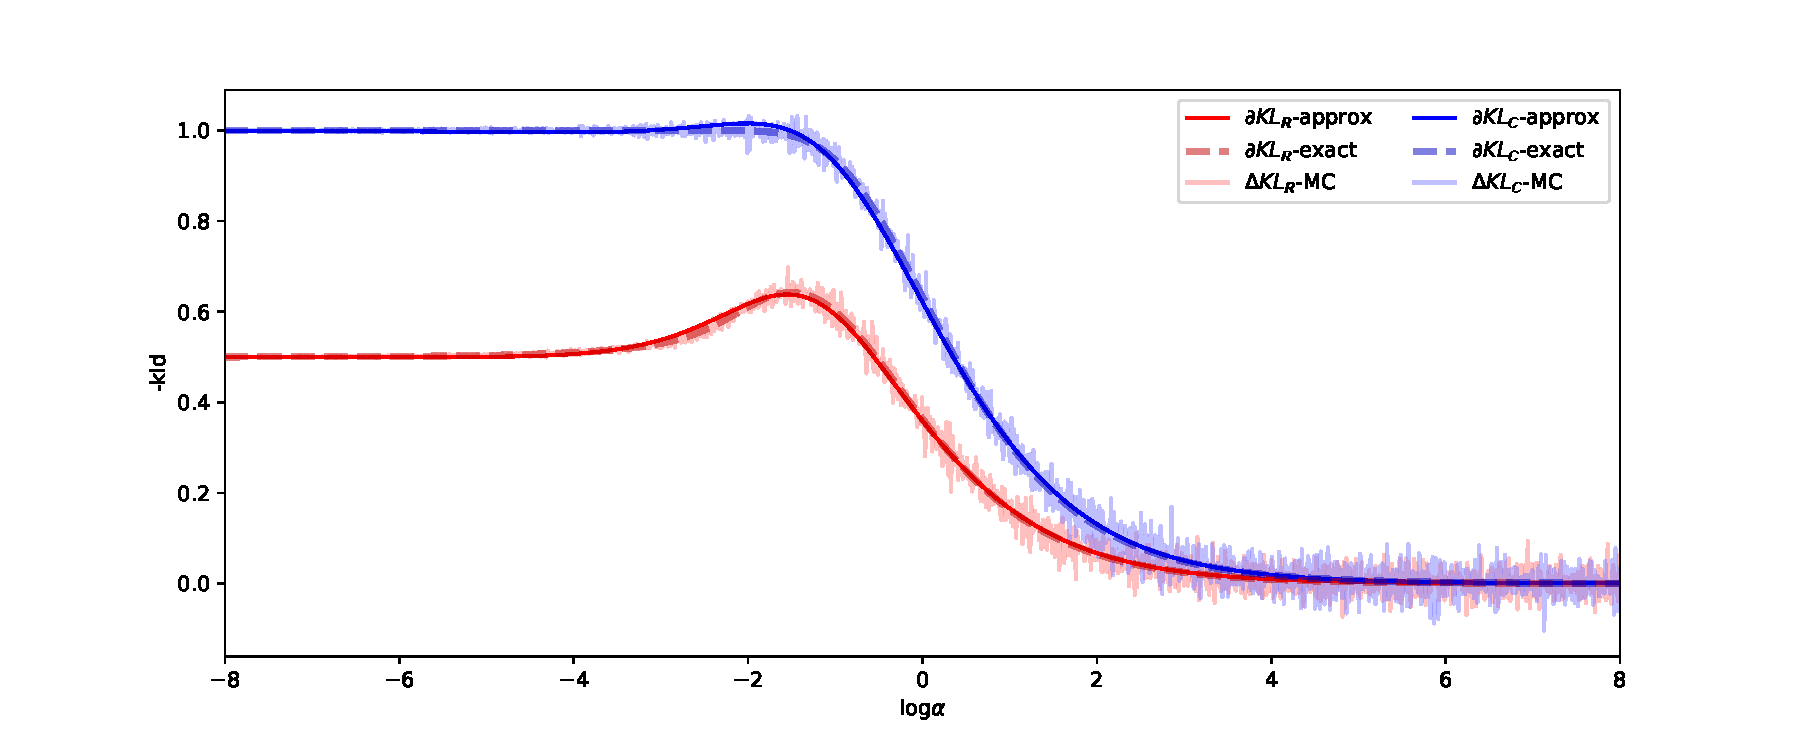
\includegraphics[width=1.\linewidth]{../notebooks/assets/grad_log.pdf}
  \caption{$\tfrac{d f(\alpha)}{d \log{\alpha}}$ of the fit \cite{molchanov_variational_2017},
  MC estimate, and exact derivative using \eqref{eq:real-kl-div-deriv-log}.}
  \label{fig:molchanov-derivative-replica}
\end{figure}

Now in SGD (and specifically in SGVB) we are concerned more with the gradient field, induced
by the potential (which is the loss function), rather than the value itself. Thus, as far as
the regularizing penalty term is concerned, which is used to regularize the loss objective,
we can essentially ignore it's forward pass value (level) and just compute its gradient
(subgradient, normal cone) with respect the parameter of interest in sgd. (unless it is a
part of a constraint, ie. downstream computation)

% subsection real-chisq-grad (end)

\subsection{Backpropagation through $\cplx$-networks} % (fold)
\label{sub:wirtinger_calculus}

% TLDR: we use Wirtinger calculus!
Following \cite{trabelsi_deep_2017}, we naturally identify $\cplx$ with $\real^2$ via $
  z_\mathrm{r} + j z_\mathrm{i} \mapsto (z_\mathrm{r}, z_\mathrm{i})
$, storing the real and imaginary parts in interleaved format, and emulate $\cplx$-algebra
using $\real$-valued arithmetic. 

% essential intro into Wirtinger calculus (CR)
% https://math.stackexchange.com/a/444493
Wirtinger ($\cplx\real$) calculus relies on the natural identification of $\cplx$ with $
  \real \times \real
$, and regards $
  f\colon \cplx \to \cplx
$ as an equivalent in algebraic sense function $F\colon \real^2 \to \cplx$ defined $
  f(z) = f(u + jv) = F(u, v)
$. Under this identification, we define two formal derivative operators
$
  \tfrac{\partial}{\partial z}
    = \tfrac12 \bigl(
      \tfrac{\partial}{\partial u}
      - j \tfrac{\partial}{\partial v}
    \bigr)
$ and $
  \tfrac{\partial}{\partial \conj{z}}
    = \tfrac12 \bigl(
      \tfrac{\partial}{\partial u}
      + j \tfrac{\partial}{\partial v}
    \bigr)
$ and the differential of $f$ at $z \in \cplx$ as
$$
df(z) \big\vert_{z=u + jv}
  = \frac{\partial f}{\partial z} dz
    + \frac{\partial f}{\partial \conj{z}} d\conj{z}
   % = \frac12\bigl(
   %    \frac{\partial}{\partial u}
   %    - j \frac{\partial}{\partial v}
   % \bigr) F (du - j dv)
   % + \frac12\bigl(
   %    \frac{\partial}{\partial u}
   %    + j \frac{\partial}{\partial v}
   % \bigr) F (du - j dv)
   % = \frac12 \bigl(
   %    \frac{\partial F}{\partial u} du - j \frac{\partial F}{\partial v} du
   %    + j \frac{\partial F}{\partial u} dv + \frac{\partial F}{\partial v} dv
   % \bigr)
   % + \frac12 \bigl(
   %    \frac{\partial F}{\partial u} du + j \frac{\partial F}{\partial v} du
   %    - j \frac{\partial F}{\partial u} dv + \frac{\partial F}{\partial v} dv
   % \bigr)
   = \frac{\partial F}{\partial u} du
     + \frac{\partial F}{\partial v} dv
   = dF(u, v)
  \,, $$
where $dz = du + j dv$ and $d\conj{z} = du - j dv$. This implies that the complex argument
and its conjugate are treated as independent variables. Cauchy-Riemann conditions $
  -j \tfrac{\partial F}{\partial v} = \tfrac{\partial F}{\partial u}
$ impose a rigid structure on real and imaginary parts of $F$ and can be expressed as $
  \tfrac{\partial f}{\partial \conj{z}} = 0
$ in this notation. Thus $\cplx\real$ calculus subsumes the usual $\cplx$-calculus on
holomorphic functions, when $f(z)$, regarded as $f(z, \conj{z})$, is constant with respect
to $\conj{z}$. The usual rules of calculus, like chain and product rules, follow directly
from the definition of the operators, e.g.
$$
  \frac{\partial (f\circ g)}{\partial z}
    = \frac{\partial f(g(z))}{\partial g} \frac{\partial g(z)}{\partial z}
    + \frac{\partial f(g(z))}{\partial \conj{g}} \frac{\partial \conj{g(z)}}{\partial z}
    % = \nabla G \nabla F
  \,. $$
% Show that $dh(z) = df(g(z)) dg(z)$.
% $h(z) = f(g(z)) = F(G_r(u, v), G_i(u, v)) = H(u, v)$
% $$
% dH
%   = \tfrac{\partial F}{\partial x} \tfrac{\partial G_r}{\partial u} du
%   + \tfrac{\partial F}{\partial x} \tfrac{\partial G_r}{\partial v} dv
%   + \tfrac{\partial F}{\partial y} \tfrac{\partial G_i}{\partial u} du
%   + \tfrac{\partial F}{\partial y} \tfrac{\partial G_i}{\partial v} dv
%   = \tfrac{\partial F}{\partial r} d\Re g(z)
%   + \tfrac{\partial F}{\partial i} d\Im g(z)
%   = df(\Re g(z) + j\Im g(z)) d g(z)
%   = df(g(z)) d g(z)
%   \,. $$

In machine learning tasks the target objective is typically empirical risk, which has to
be real-valued to be minimized. Nevertheless, the expression of the $\cplx\real$ gradient
is compatible with what is expected, when $f$ is treated like a $\real^2$ function. For a
real-valued $f\colon \cplx \to \real$ we have $\conj{f} = f$, which implies $
  \tfrac{\partial f}{\partial \conj{z}}
    = \tfrac{\partial \conj{f}}{\partial \conj{z}}
    = \conj{\tfrac{\partial f}{\partial z}}
$, whence
$$
df
  = \tfrac{\partial f}{\partial z} dz
    + \tfrac{\partial f}{\partial \conj{z}} d\conj{z}
  % = \conj{\tfrac{\partial \conj{f}}{\partial \conj{z}}} dz
  % + \conj{\conj{\tfrac{\partial f}{\partial \conj{z}}} dz}
  = 2 \Re \Bigl(
    \conj{\tfrac{\partial f}{\partial \conj{z}}} dz
  \Bigr)
  = 2 \Re \bigl(
    \tfrac{\partial f}{\partial z} dz
  \bigr)
  \,. $$
Thus, the gradient of $f$ at $z$ is given by $
  \nabla_z f(z)
    = \tfrac{\partial F}{\partial u}
      + j \tfrac{\partial F}{\partial v}
$. Therefore, Wirtinger calculus makes it possible to reuse $\real$-backpropagation.

% subsection wirtinger_calculus (end)

\subsection{$\cplx$-Linear operator representation} % (fold)
\label{sub:c-linear_operator_representation}

% proof that such operators exist and are unique (well this is an obvious statement)
Consider $L \colon \cplx^m \to \cplx^n$ -- linear in $\cplx$. Then $
  L(u + jv) = L u + j L v
$ for any $u, v \in \real^m$, which implies that the effect of $L$ as $\cplx$-linear
operator is determined by its restriction onto $\real^n$. Let $
  F = L\vert_{\real^m}
  \colon \real^m \to \cplx^n
$ and observe that $F_r = \Re \circ F$ and $F_i = \Im \circ F$ are $\real$-linear operators
such that $F = F_r + j F_i$ (pointwise). Indeed,
$$
  F_r(a + \lambda b)
  % = \Re F(a + \lambda b)
  = \Re L(a + \lambda b)
  % = \Re \bigl( L a + \lambda L b \bigr)
  = \Re L a + \lambda \Re L b
  % = \Re F a + \lambda \Re F b
  = F_r a + \lambda F_r b
  \,. $$
Therefore for any $\cplx$-linear operator $L$ there are $\real$-linear operators $U, V$
such that
$$
L z 
  = (U + j V) (\Re z + j \Im z)
  % = (U + j V) \Re z + j (U + j V) \Im z
  % = U \Re z + j V \Re z + j \bigl(U \Im z + j V \Im z \bigr)
  = U \Re z - V \Im z + j \bigl( V \Re z + U \Im z \bigr)
  % = (U + j V) z
  \,. $$
Uniqueness of these operators follows, if this decomposition is applied to any $z$ with
$\Im z = 0$.

% subsection c-linear_operator_representation (end)

\subsubsection{MGF of a noncentral $\chi^2$} % (fold)
\label{ssub:mgf_of_a_noncentral_chi}

Consider the mgf of $W$:
$$
M_W(t)
  = \mathbb{E}(e^{Wt})
  = \prod_i \mathbb{E}(e^{(\mu_i + z_i)^2 t})
  \,, $$
by independence. Now for $z \sim \mathcal{N}(\mu, 1)$
$$
\mathbb{E}(e^{z^2 t})
  = \tfrac1{\sqrt{2\pi}}
  \int_{-\infty}^{+\infty}
      e^{z^2 t} e^{-\tfrac{(z-\mu)^2}2}
  dz
  \,. $$
Now, for $t < \tfrac12$
$$
z^2 t - \tfrac{(z - \mu)^2}2
  = - \tfrac12 (1 - 2t) z^2 + z \mu - \tfrac{\mu^2}2
  % = - \tfrac12 (1 - 2t) \bigl(
  %   z^2 - 2 z \tfrac\mu{1 - 2t} + \tfrac{\mu^2}{1 - 2t}
  % \bigr)
  % = - \tfrac12 (1 - 2t) \bigl( z - \tfrac\mu{1 - 2t} \bigr)^2
  % - \tfrac12 (1 - 2t) \bigl(
  %   \tfrac{\mu^2}{1 - 2t}
  %   - \tfrac{\mu^2}{(1 - 2t)^2}
  % \bigr)
  % = - \tfrac12 (1 - 2t) \bigl( z - \tfrac\mu{1 - 2t} \bigr)^2
  %   - \tfrac{\mu^2}2 \bigl(
  %   \tfrac{1 - 2t}{1 - 2t} - \tfrac1{1 - 2t}
  % \bigr)
  % = - \tfrac12 (1 - 2t) \bigl( z - \tfrac\mu{1 - 2t} \bigr)^2
  %   + \tfrac{\mu^2}2 \tfrac{2t}{1 - 2t}
  = - \tfrac12 (1 - 2t) \bigl( z - \tfrac\mu{1 - 2t} \bigr)^2
    + \mu^2 \tfrac{t}{1 - 2t}
  \,, $$
whence
\begin{multline}
  \mathbb{E}(e^{z^2 t})
    = \tfrac1{\sqrt{2\pi}}
      \int_{-\infty}^{+\infty}
        e^{z^2 t} e^{-\tfrac{(z-\mu)^2}2}
      \, dz
    % = e^{\mu^2 \tfrac{t}{1 - 2t}}
    %   \tfrac1{\sqrt{2\pi}}
    %   \int_{-\infty}^{+\infty}
    %     e^{- \tfrac12 (1 - 2t) \bigl( z - \tfrac\mu{1 - 2t} \bigr)^2}
    %   \, dz
    \\= e^{\mu^2 \tfrac{t}{1 - 2t}}
      \tfrac1{\sqrt{2\pi}}
      \int_{-\infty}^{+\infty}
        e^{- \tfrac12 (1 - 2t) z^2}
      \, dz
    % = [u = \sqrt{1 - 2t} z]
    % = e^{\mu^2 \tfrac{t}{1 - 2t}}
    %   \tfrac1{\sqrt{2\pi}}
    %   \int_{-\infty}^{+\infty}
    %     e^{- \tfrac12 u^2}
    %   \, \tfrac{du}{\sqrt{1 - 2t}}
    = \tfrac{
        \exp{\{\mu^2 \tfrac{t}{1 - 2t}\}}
    }{\sqrt{1 - 2t}}
    \,.
\end{multline}
Therefore
$$
M_W(t)
  = \mathbb{E}(e^{Wt})
  = \prod_i \tfrac{
      e^{\mu_i^2 \tfrac{t}{1 - 2t}}
    }{\sqrt{1 - 2t}}
  % = e^{\lambda \tfrac{t}{1 - 2t}}
  %   (1 - 2t)^{-\tfrac{m}2}
  % = e^{\lambda \tfrac{- t}{2t - 1}}
  %   (1 - 2t)^{-\tfrac{m}2}
  % = e^{\tfrac\lambda2 \tfrac{1 - 2t - 1}{2t - 1}}
  %   (1 - 2t)^{-\tfrac{m}2}
  % = e^{- \tfrac\lambda2 (1 + \tfrac1{2t - 1})}
  %   (1 - 2t)^{-\tfrac{m}2} 
  = e^{- \tfrac\lambda2} e^{\tfrac\lambda2 \tfrac1{1 - 2t}}
  (1 - 2t)^{-\tfrac{m}2}
  \,. $$
Expanding the exponential as infinite series:
\begin{multline}
  M_W(t)
    = e^{- \tfrac\lambda2} e^{\tfrac\lambda2 \tfrac1{1 - 2t}}
    (1 - 2t)^{-\tfrac{m}2}
    % = e^{- \tfrac\lambda2} (1 - 2t)^{-\tfrac{m}2}
    %   \sum_{n \geq 0} \tfrac{\bigl(\tfrac\lambda2\bigr)^n}{n! (1 - 2t)^n}
    \\= \sum_{n \geq 0} \tfrac{e^{- \tfrac\lambda2} \bigl(\tfrac\lambda2\bigr)^n}{n!}
        (1 - 2t)^{-\tfrac{2n + m}2}
    = \sum_{n \geq 0} \tfrac{e^{- \tfrac\lambda2} \bigl(\tfrac\lambda2\bigr)^n}{n!}
        \mathbb{E}_{x \sim \chi^2_{m + 2n}}(e^{x t})
    \,.
\end{multline}

% subsubsection mgf_of_a_noncentral_chi (end)

% section appendix (end)

%%%%%%%%%%%%%%%%%%%%%%%%%%%%%%%%%%%%%%%%%%%%%%%%%%%%%%%%%%%%%%%%%%%%%%%%%%%%%%%%%%%%%%%%%%%%%%%%%%%

\clearpage


\section{Trunk} % (fold)
\label{sec:trunk}



In a fully Bayesian treatment, the dropout rate $p$, which governs the regularization strength,
would appear in the KL-divergence term of ELBO \eqref{eq:elbo} through the corresponding odds 
ratio $
  \alpha = \tfrac{p}{1-p}
$, which.

it vary on the per-parameter basis, which allows for even more flexible posterior
approximations.

% revirew of kingma and lrt
The key contributions of \cite{kingma_variational_2015} are reinterpretation of dropout
as a variational inference method

that optimizes the $\log$-likelihood term from the Evidence Lower Bound.

 % who proposed sparsification?



In the case of $\real$-valued variational dropout \cite{kingma_variational_2015} approximate
\eqref{eq:expect-improper-term-cplx} by a non-linear regression, fit to the Monte-Carlo estimates
of the expectation for $\alpha$ varying over a logarithmic grid. This approximation was greatly
refined in \cite{molchanov_variational_2017} -- an improvement that enabled doing away with
the clipping of the dropout rate (relevance score) $\alpha$. In fact in the real case the analogue
of the last term in \eqref{eq:expect-improper-term-cplx} is half the log-moment of a non-central
$\chi^2$ distribution with shape $1$ and non-centrality $\lambda = \tfrac1{\alpha}$. Unfortunately,
there is no known expression (even involving special functions) for this expectation for
$\chi^2_m$ with odd shape parameter $m$ (degrees of freedom) \verify{this}. Quite fortunately
there is one for even degrees of freedom.

%%%%%%%
\todo{why this is better than a general $\cplx$-gaussian? Three parameters?}

\important{``pytorch'' specific}
Otherwise we have to offload the values from the device to cpu, compute the special
function there, and transfer back.

Why sparsity matters, why $\cplx$ networks?

Where are $\cplx$-networks used? and do these applications warrant sparsity?

Gist of the LRP (\cite{kingma_variational_2015})
translating uncertainty (randomness) from parameters to activations
  adds noise -- helps regularization
  emulates one draw per batch element -- decorrelates gradient within the batch
  reduces computations (memory), leverages batched matmuls (or convos)
  decreases variance of the gradient

additive noise reparameterization (molchanov\_variational\_2017) $(\mu, \alpha \mu^2)$:
  less noisy gradient wrt $\mu$, $\alpha$ recomputed on-the-fly

\subsection{$\cplx$-valued networks} % (fold)
\label{sub:c_valued_networks}

In this section i remind the reader what the complex-valued networks are, how
they are implemented and how much of $\cplx$-ness they have. Mention careful
design.

I will describe the linear layers (dense, masked, and convolutions) and
activations borrowed straight from the $\real$-values networks. Then i shall
mention that this has been tried before and list papers that one way or another
address $\cplx$-data processing with neural networks.


It is worth pointing out that the key advantage of
the $\cplx$-constraints is that they permit use of Strassen's $3$M multiplication algorithm,
potentially \verify{saving up} to $25\%$ on floating point multiplications. \todo{
  in contrast to what? to na{\:i}ve (obvious)? to paired-$\real$ ($2 \times 2$-$2\times 1$
  -- 4 fmul)?
}

% subsection c_valued_networks (end)

\section{Bayesian methods} % (fold)
\label{sec:bayesian_methods}

In this section we outline and derive the variational dropout technique for complex-%
valued networks, which re-traces the evolution of dropout technique for real-valued
weights.

% a second take on bayesian inference
The core question of Bayesian analysis is concerned with the distribution of the data model
after observing data and given the initial belief about it. The data model is typically a joint
distribution on the sample, which includes assumptions regarding independence and (conditional)
factorization of the distribution of each individual data point. In our case we suppose that
the data $
  \mathcal{D} = (z_i)_{i=1}^m
$, $z_i = (x_i, y_i)$ is independent and identically distributed under our model $m$: $
  p(\mathcal{D}\mid m)
    = \prod_i p(z_i\mid m)
$. The models we  our model $m$ comes from a parametric conditional distribution family, e.g. $
  p(z \mid m)
    = p(y \mid x, m) p(x \mid m)
    = p(y \mid x, m) p(x)
$ and $
  p(y \mid x, m)
    = \mathcal{N}\bigl(
      y\,\mid\, \mu_\omega(x)\,, \sigma^2_\omega(x)
    \bigr)
$, then we can (and do) identify $m$ with its parameters $\omega$. Instead of iid data in
$\mathcal{D}$, we could have assumed a Gaussian Process data model $
  y(x) \sim \mathrm{GP}(\mu, K)
$ for the mean function and covariance kernel $
  \mu
    \colon \mathcal{X} \to \real^d
$ and $
  K \colon \mathcal{X} \times \mathcal{X}
    \to \real^{d\times d}
$.

In the framework of Bayesian Inference we use the Bayes's rule as an exact method for deriving
the posterior parameter distribution from the likelihood of the data model and model's prior:
$
  p(\omega \mid \mathcal{D})
    = \tfrac{
      p(\mathcal{D} \mid \omega) \pi(\omega)
    }{
      p(\mathcal{D})
    }
$. Typically, exact inference involves an analytically intractable integrals, e.g. in the
denominator of the posterior $
  p(\mathcal{D})
    = \int p(\mathcal{D} \mid \omega) \pi(\omega) d\omega
$, or derived distributions, such as the predictive distribution $
  p(y \mid x, \mathcal{D})
    = \int p(y \mid x, \omega) p(\omega \mid \mathcal{D}) d\omega
$.

Variational Inference recasts the problem of posterior derivation into functional optimization
framework. The main idea is to find the closest approximation to the posterior $
  p(\omega \mid \mathcal{D})
$ in some family $
  \mathcal{Q}
$ of approximating distributions $
  q(\omega)
$ on the parameters $\omega$ of the model $m$ (or the model itself). The proximity between
distributions is measured either using MMD metric via embedding into some universal RKHS,
\cite{citation_needed}, Wasserstein \cite{citation_needed} \cite{citation_needed}, total
variation norm \cite{citation_needed}, or $f$-divergences
% $
%   \mathbb{E}_{\omega \sim q(\omega)} f\bigl(
%       \tfrac{p(\omega)}{q(\omega)}
%     \bigr)
% $ for a convex $f$ with $f(1) = 0$
\cite{citation_needed}, specifically Kullback-Leibler divergence. The key trade off in Variational
Inference is the choice of the approximating family that is rich enough to get close to the true
posterior, yet simple enough to sample from or for inferring derived distributions via Bayesian
averaging.

Despite the effort to simplify the bayesian analysis in the most commonly encountered cases
variational inference still requires dealing with analytically intractable expectations,
\cite{citation_needed}. This issue is dealt with by giving up deterministic precision to
gain efficiency from stochastic, since inaccuracies and assumptions are inevitable, especially
when modelling observations.

% a verbatim setion from my mlss2019 bdl notebook
In Bayesian Inference (\textbf{BI}) we \textit{assume} that the observation data $D$ follows a
\textit{model} $m$ with data generating distribution $p(D \mid m, \omega)$ \textit{governed by
unknown parameters} $\omega$. The goal of \textbf{BI} is to reason about the model and/or its
parameters, and new data given the observed data $D$ and our assumptions, i.e to seek the
\textbf{posterior} parameter and predictive distributions:

\begin{align}
p(d \mid D, m)
  &
  % = \mathbb{E}_{
  %   \omega \sim p(\omega \mid D, m)
  % } p(d \mid D, \omega, m)
  = \int p(d \mid D, \omega, m) p(\omega \mid D, m) d\omega
  \,, \\
p(\omega \mid D, m)
  &
  = \frac{p(D \mid \omega, m) \, \pi(\omega \mid m)}{p(D \mid m)}
  \,,
\end{align}
where
\begin{itemize}
  \item the \textbf{prior} distribution $\pi(\omega \mid m)$ reflects our belief before
  having made the observations
  \item the data distribution $p(D \mid \omega, m)$ reflects our assumptions about the data
  generating process, and determines the model \textbf{likelihood} (Gaussian, Categorical,
  Poisson etc.)
\end{itemize}
Unless the distributions and likelihoods are conjugate, posterior in Bayesian inference is
typically intractable and it is common to resort to \textbf{Variational Inference} or
\textbf{Monte Carlo} approximations.

Since inference using the exact posterior is rarely tractable, efficient and unbiased approximation
schemes are typically used. One such scheme is Variational Inference, which casts the inference
task into the domain of optimization problems over some appropriately chosen the posterior
distribution approximation family. The key idea of the former is to seek an approximation
$q(\omega)$ to the intractable posterior $p(\omega \mid D, m)$, via a variational optimization
problem over some parametric family of distributions $\mathcal{Q}$:
$$
q^*(\omega)
    \in \arg \min_{q\in \mathcal{Q}}
      \mathrm{KL}(q(\omega) \| p(\omega \mid D, m))
  \,, $$
where the Kullback-Leibler divergence between $P$ and $Q$ ($P\ll Q$) with densities $p$ and $q$,
respectively, is given by
$$
\mathrm{KL}(q(\omega) \| p(\omega))
  % = \mathbb{E}_{\omega \sim Q} \log \tfrac{dQ}{dP}(\omega)
  = \mathbb{E}_{\omega \sim q(\omega)}
    \log \tfrac{q(\omega)}{p(\omega)}
  \,.
  % \tag{kl-div}
  $$

Note that the family of variational approximations $\mathcal{Q}$ can be structured
\textbf{arbitrarily}: point-mass, products, mixture, dependent on input, having mixed hierarchical
structure, -- any distribution, even unnormalized. Although computing the divergence w.r.t.
the unknown posterior is still hard and intractable, it is possible to do away with it
through the following identity, which is based on the Bayes rule.

For \textbf{any} $q(\omega) \ll p(\omega \mid D; \phi)$ and any model $m$

\begin{align}
\overbrace{
  \log p(D \mid m)
}^{\text{evidence}}
  &= \overbrace{
    \mathbb{E}_{\omega \sim q} \log p(D\mid \omega, m)
  }^{\text{expected conditional likelihood}}
  - \overbrace{
    \mathrm{KL}(q(\omega)\| \pi(\omega \mid m))
  }^{\text{proximity to prior belief}}
  \\
  &+ \underbrace{
    \mathrm{KL}(q(\omega)\| p(\omega \mid D, m))
  }_{\text{posterior approximation}}
\,.
\tag{master-identity}
\end{align}
Instead of minimizing the divergence of the approximation from the posterior, we can maximize
the \textbf{Evidence Lower Bound} with respect to $q(\omega)$:
$$
q^* \in
  \arg\max_{q\in Q}
    \mathcal{L}(q)
    = \mathbb{E}_{\omega \sim q} \log p(D\mid \omega, m)
      - \mathrm{KL}(q(\omega)\| \pi(\omega \mid m))
  \,.
  % \tag{max-ELBO}
  $$
The intuition is that the expected $\log$-likelihood favours $q$ that place their mass on
parameters $\omega$ that explain $D$ under the specified model $m$. At the same time
the negative KL-divergence discourages the approximation $q$ from straying too far away
from to the prior belief $\pi$ under $m$.

We usually consider the following setup (conditioning on model $m$ is omitted):
\begin{itemize}
  \item the likelihood factorizes $
    p(D \mid \omega)
        = \prod_i p(y_i, x_i \mid \omega)
        \propto \prod_i p(y_i \mid x_i, \omega)
  $
  for $D = (x_i, y_i)_{i=1}^N$

  \item the variational posterior approximation is parameterized by $\theta$: $q(\omega \mid \theta)$

  \item the prior on $\omega$ also depends on hyper-parameters $\lambda$, that can be fixed,
  or variable ($\pi(\omega \mid \lambda)$).
\end{itemize}

In this case the variational objective (evidence lower bound)
$$
\log p(D\mid \lambda )
  \geq \mathcal{L}(\theta, \lambda)
    = \mathbb{E}_{\omega \sim q(\omega \mid \theta)}
      \sum_i \log p_\phi(y_i \mid x_i, \omega)
    - KL(q(\omega \mid \theta) \| \pi(\omega \mid \lambda))
  \,, $$
is maximized with respect to $\theta$ (to approximate the posterior).

Priors can be
\begin{itemize}
  \item \textit{subjective}, i.e. reflecting prior beliefs (but not arbitrary)
  \item \textit{objective}, i.e. reflecting our lack of knowledge
  \item \title{empirical}, i.e. learnt from the observed data (optimized over
  hyper-parameters $\lambda$)
\end{itemize}

The stochastic variant of ELBO is formed by randomly batching
the dataset $D$:
$$
\mathcal{L}(\theta, \lambda)
  \approx \mathcal{L}_\mathrm{SGVB}(\theta, \lambda)
  = \lvert D \rvert \biggl(
    \tfrac1{\lvert B \rvert}
      \sum_{b \in B} \mathbb{E}_{\omega \sim q(\omega \mid \theta)}
        \log p(y_b \mid x_b, \omega)
  \biggr)
  - KL(q(\omega \mid \theta) \| \pi(\omega \mid \lambda))
  \,. $$

Stochastic optimization follows noisy unbiased gradient estimates, which are usually cheap and
allow escaping from local optima, but optimize the objective in expectation. In order to get
a gradient of $
  F_\theta = \mathbb{E}_{\omega \sim q(\omega \mid \theta)} f(\omega)
$ w.r.t $\theta$ we use either:
\begin{itemize}
  \item (REINFORCE) $
    \nabla_\theta F_\theta
      = \mathbb{E}_{\omega \sim q(\omega \mid \theta)}
        (f(\omega) - b_\theta) \nabla_\theta \log q(\omega \mid \theta)
  $ for some $b_\theta$ that is used to control variance

  \item (reparameterization) $
    \nabla_\theta F_\theta
      = \nabla_\theta \mathbb{E}_{\varepsilon \sim q(\varepsilon)}
        f(g(\theta; \varepsilon))
      = \mathbb{E}_{\varepsilon \sim q(\varepsilon)}
        \nabla_\theta g(\theta; \varepsilon)
          \nabla_\omega f(\omega) \big\vert_{\omega = g(\theta; \varepsilon)}
    $ when there are $q$ and differentiable $g$, such that sampling from $
      q(\omega \mid \theta)
    $ is equivalent to $
      \omega = g(\theta; \varepsilon)
    $ with $\varepsilon \sim q(\varepsilon)$
\end{itemize}

The variational approximation might yield high dimensional integrals, which are slow/prohibitive
to compute. To make the computations faster without foregoing much of the precision, we may use
Monte Carlo estimator:
$$
\mathbb{E}_{\omega \sim q(\omega\mid \theta)} \, f(\omega)
  \overset{\text{MC}}{\approx}
    \frac1{\lvert \mathcal{W}\rvert}
      \sum_{\omega \in \mathcal{W}} f(\omega)
  \,, $$
where $\mathcal{W} = (\omega_b)_{b=1}^B$ is a sample of independent draws from $
  q(\omega\mid \theta)
$. If we also approximate the expectation wrt model parameters in the gradient of ELBO via Monte
Carlo we get the \textbf{doubly stochastic variational objective}:
$$
\nabla_\theta \mathcal{L}_\mathrm{DSVB}(\theta, \lambda)
  \approx
    \lvert D \rvert \biggl(
      \tfrac1{\lvert B \rvert}
        \sum_{b \in B}
          \mathop{gradient}(x_b, y_b)
    \biggr)
    - \nabla_\theta KL(q(\omega \mid \theta) \| \pi(\omega \mid \lambda))
  \,, $$
where `gradient` is $
  \nabla_\theta
    \mathbb{E}_{\omega \sim q(\omega \mid \theta)}
      \log p(y \mid x, \omega)
$ using one of the approaches above, typically approximated using one independent draw of $\omega$
per $b\in B$. We can use a similar sampling approach to compute the gradient of the divergence term.

We can estimate the divergence term in the ELBO with Monte Carlo, or, for example, for the
predictive distribution we have
\begin{align}
\mathbb{E}_{y\sim p(y\mid x, D, m)} \, g(y)
  &
  \overset{\text{BI}}{=}
    \mathbb{E}_{\omega\sim p(\omega \mid D, m)}
      \mathbb{E}_{y\sim p(y\mid x, \omega, D, m)} \, g(y)
  \\
  &
  \overset{\text{VI}}{\approx}
    \mathbb{E}_{\omega\sim q(\omega)}
      \mathbb{E}_{y\sim p(y\mid x, \omega, D, m)} \, g(y)
  \\
  &
  \overset{\text{MC}}{\approx}
    % \hat{\mathbb{E}}_{\omega \sim \mathcal{W}}
    %   \mathbb{E}_{y\sim p(y\mid x, \omega, D, m)} \, g(y)
    \frac1{\lvert \mathcal{W}\rvert} \sum_{\omega \in \mathcal{W}}
      \mathbb{E}_{y\sim p(y\mid x, \omega, D, m)} \, g(y)
  \,,
\end{align}
where $\mathcal{W} = (\omega_b)_{b=1}^B \sim q(\omega)$ -- iid samples from the variational
approximation.

\bigskip

% on bernoulli dropout
Bernoulli dropout alleviates the problem of overfitting

% a comment on Bernoulli dropout
The key idea of Bernoulli dropout is to randomly mask input features of a layer during
training with in order to learn decorrelated feature maps. In a recent study of network
capacity for multitask learning, \cite{multitask2019}, it was shown, that associating
each dataset (task) with a context, that masks a subset of the parameters, allows non-%
destructive `packing' of the tasks in orthogonal on average `subsets' of a single set
of weights, without much interference between tasks. This lends support for beneficial
effects of Bernulli Dropout on test performance, since, in effect, the network learns
to perform well on identical copies of the same task with different (binary) contexts
with a single parameter set.

% on gaussian dropout

The local reparameterization trick, proposed by \cite{citation_wang_menning_2013} in the context
of Bernoulli and Gaussian dropout regularization techniques \cite{citation_needed}, translates
the uncertainty about global parameters to noise in the local intermediate state and utilizes
the closure of Gaussian distribution under affine transformations. Computational advantage of
the trick is that activation noise is cheaper to sample and store for the purposes of backpropagation,
than independently sampling parameters from the posterior approximation individually for each
element of the minibatch. As far as Bayesian inference is concerned, \cite{kingma_variational_2015}
have shown that trick's beneficial effects on minibatch SGD convergence come via two mechanisms
of likelihood gradient estimator's efficiency: decorrelation within the batch (independent noise
draws) and variance reduction through local transfer of parameter uncertainty to activation noise.

\begin{quote}

in practice the performance of stochastic gradient methods depends on the variance of the gradient
field

sampling the activations directly, without the parameter randomness gives a low cost efficient
MC estimator (statistical efficiency).

the gradient in sgvb is unbiased estimate of the $\log$-likelihood part of the elbo

\end{quote}

A linear layer is parameterized by $W \in\real^{n \times m}$ and bias $b\in \real^n$ and
acts on its input $x\in \real^m$ via $y = W x + b$ with $y\in \real^n$. The key idea of
Bernoulli dropout is to mask elements in the matrix $W$ of the layer
with some given probability $p$: $W = \theta \odot \xi$ with $\theta$ being the learnt
weight matrix, and $
  \xi \sim \mathcal{B}(\{0, \tfrac1{1-p}\}, 1-p)
$ -- an iid Bernoulli mask. During training, a dropout mask $\xi$ is used to compute $W$,
and during evaluation the weights are fixed to the expectation of $W$ which is $\theta$.
The discussion and analysis in \cite{kingma_variational_2015}, suggest that drawing one
common dropout mask for all data in the minibatch reduces statistical efficiency the estimator
of the weights' gradient in the stochastic approximation of the evidence lower bound. 

Gaussian dropout works in a similar fashion, except the dropout mask $\xi$ is iid $
  \mathcal{N}(1, \alpha=\tfrac{p}{1-p})
$, i.e. a multiplicative Gaussian noise is injected into the network.

The key idea of Variational Dropout is to assume a Gaussian Mean field variational
approximation of the posterior distribution of linear layer's weights (or convolutional
kernels, with a caveat\footnote).  \footnotetext{
  at each spatial patch of input data the kernel is independently redrawn form the
  VI distribution. This again helps with gradient variance reduction.
}
Weight $W$ are assumed to have independently distributed elements with $
  w_{ij} \sim \mathcal{N}(\theta_{ij}, \sigma^2_{ij})
$.

In fact multiplicative Gaussian dropout on weights $W$ is in fact itself a variational
approximation with variance $\sigma^2_{ij} = \theta_{ij}^2 \tfrac{p}{1-p}$ determined
by the dropout rate.


% set by step we retell the story of kingma_variational_2015
Gaussian variational approximation enabled \cite{kingma_variational_2015} propose a
\textit{local reparameterization trick}, which reduces the variance of the gradients
in SGVB and does not resample $W$ per element of a minibatch. It relies the closure
of Gaussian distribution under linear transformations. Indeed, if $W$ is a Gaussian
matrix with independently distributed $
  W_{ij} \sim \mathcal{N}(\theta_{ij}, \sigma^2_{ij})
$, then we have \important{moved}.



and instead
translating the uncertainty from the weights into local output noise of each linear layer.
Without this it would have been necessary to draw new set of random weights per each element
in a mini-batch.

$$
  \mathcal{N}(\theta_{ij}, \alpha \theta^2_{ij})
  \overset{\mathcal{D}}{\sim}
  \theta_{ij} \mathcal{N}(1, \alpha)
  \,, $$

\cite{molchanov_variational_2017} propose additional step in the local reparametrization,
which further reduces the variance of the gradient estimator for each dropped out
weight. Their simple formal change of variables $(\theta, \alpha) \to (\theta, \sigma^2)$
decouples the stochastic component from the weights \rewrite:
$$
  w_{ij} = \theta_{ij} + \theta_{ij} \sqrt{\alpha} \varepsilon_{ij}
  \,\to\,
  w_{ij} = \theta_{ij} + \sigma^2_{ij} \varepsilon_{ij}
  \,, $$
with the appropriate change of variables in the Kullback-Leibler divergence.
($\alpha_{ij} = \tfrac{\sigma_{ij}^2}{\lvert \theta_{ij}\rvert^2}$).

Criticism of \cite{gale_state_2019} implies that $\ell_0$-variational dropout,
proposed by \cite{louizos_learning_2017} and based on the concrete binary distribution
of \cite{maddison_concrete_2016}, works consistently better than the variational
Gaussian dropout.

The expectation in \eqref{eq:expect-improper-term-cplx} involves a log-moment of the non-central
$\chi^2_2$ distribution, which has an analytic expression for the gradient, unlike the case
in $\real$-dropout penalty \eqref{eq:improper-kl-div-real}.

% section bayesian_methods (end)

\end{document}